\documentclass[a4paper]{book}
\usepackage{a4wide}
\usepackage{makeidx}
\usepackage{graphicx}
\usepackage{multicol}
\usepackage{float}
\usepackage{listings}
\usepackage{color}
\usepackage{textcomp}
\usepackage{alltt}
\usepackage{times}
\usepackage{ifpdf}
\ifpdf
\usepackage[pdftex,
            pagebackref=true,
            colorlinks=true,
            linkcolor=blue,
            unicode
           ]{hyperref}
\else
\usepackage[ps2pdf,
            pagebackref=true,
            colorlinks=true,
            linkcolor=blue,
            unicode
           ]{hyperref}
\usepackage{pspicture}
\fi
\usepackage[utf8]{inputenc}
\usepackage{doxygen}
\lstset{language=C++,inputencoding=utf8,basicstyle=\footnotesize,breaklines=true,breakatwhitespace=true,tabsize=8,numbers=left }
\makeindex
\setcounter{tocdepth}{3}
\renewcommand{\footrulewidth}{0.4pt}
\begin{document}
\hypersetup{pageanchor=false}
\begin{titlepage}
\vspace*{7cm}
\begin{center}
{\Large Encrypted Facebook \\[1ex]\large 0.1 }\\
\vspace*{1cm}
{\large Generated by Doxygen 1.7.1}\\
\vspace*{0.5cm}
{\small Sun Jan 2 2011 06:39:40}\\
\end{center}
\end{titlepage}
\clearemptydoublepage
\pagenumbering{roman}
\tableofcontents
\clearemptydoublepage
\pagenumbering{arabic}
\hypersetup{pageanchor=true}
\chapter{Namespace Index}
\section{Namespace List}
Here is a list of all documented namespaces with brief descriptions:\begin{DoxyCompactList}
\item\contentsline{section}{\hyperlink{namespacecimg__library}{cimg\_\-library} (This namespace encompasses all classes and functions of the CImg library )}{\pageref{namespacecimg__library}}{}
\item\contentsline{section}{\hyperlink{namespacecimg__library_1_1cimg}{cimg\_\-library::cimg} (Namespace that encompasses {\itshape low-\/level\/} functions and variables of the CImg Library )}{\pageref{namespacecimg__library_1_1cimg}}{}
\end{DoxyCompactList}

\chapter{Class Index}
\section{Class Hierarchy}
This inheritance list is sorted roughly, but not completely, alphabetically:\begin{DoxyCompactList}
\item \contentsline{section}{CImg$<$ T $>$}{\pageref{structcimg__library_1_1CImg}}{}
\item \contentsline{section}{CImg$<$ char $>$}{\pageref{structcimg__library_1_1CImg}}{}
\begin{DoxyCompactList}
\item \contentsline{section}{DataCarrierImg}{\pageref{structDataCarrierImg}}{}
\end{DoxyCompactList}
\item \contentsline{section}{CImgDisplay}{\pageref{structcimg__library_1_1CImgDisplay}}{}
\item \contentsline{section}{CImgException}{\pageref{structcimg__library_1_1CImgException}}{}
\item \contentsline{section}{CImgList$<$ T $>$}{\pageref{structcimg__library_1_1CImgList}}{}
\end{DoxyCompactList}

\chapter{Class Index}
\section{Class List}
Here are the classes, structs, unions and interfaces with brief descriptions:\begin{DoxyCompactList}
\item\contentsline{section}{\hyperlink{classefb_1_1BotanCrypto}{BotanCrypto$<$ N, M $>$} (Botan cryptography class using N-\/byte AES and M-\/byte RSA )}{\pageref{classefb_1_1BotanCrypto}}{}
\item\contentsline{section}{\hyperlink{structefb_1_1ConduitImageExractException}{ConduitImageExractException} }{\pageref{structefb_1_1ConduitImageExractException}}{}
\item\contentsline{section}{\hyperlink{structefb_1_1ConduitImageImplantException}{ConduitImageImplantException} }{\pageref{structefb_1_1ConduitImageImplantException}}{}
\item\contentsline{section}{\hyperlink{classefb_1_1Core}{Core} }{\pageref{classefb_1_1Core}}{}
\item\contentsline{section}{\hyperlink{structefb_1_1ExractException}{ExractException} }{\pageref{structefb_1_1ExractException}}{}
\item\contentsline{section}{\hyperlink{structefb_1_1FacebookId}{FacebookId} }{\pageref{structefb_1_1FacebookId}}{}
\item\contentsline{section}{\hyperlink{structefb_1_1FecDecodeException}{FecDecodeException} }{\pageref{structefb_1_1FecDecodeException}}{}
\item\contentsline{section}{\hyperlink{structefb_1_1FecEncodeException}{FecEncodeException} }{\pageref{structefb_1_1FecEncodeException}}{}
\item\contentsline{section}{\hyperlink{classefb_1_1HaarConduitImage}{HaarConduitImage} }{\pageref{classefb_1_1HaarConduitImage}}{}
\item\contentsline{section}{\hyperlink{classefb_1_1IConduitImage}{IConduitImage} (Abstract class defining a conduit image, with functionality for implanting and extracting data )}{\pageref{classefb_1_1IConduitImage}}{}
\item\contentsline{section}{\hyperlink{classefb_1_1ICore}{ICore} (\hyperlink{classefb_1_1Core}{Core} library class )}{\pageref{classefb_1_1ICore}}{}
\item\contentsline{section}{\hyperlink{classefb_1_1ICrypto}{ICrypto} (Abstract class definining the interface for the cryptographic algorithms )}{\pageref{classefb_1_1ICrypto}}{}
\item\contentsline{section}{\hyperlink{classefb_1_1IFec}{IFec} (Abstract class definining the interface for the error correction algorithms )}{\pageref{classefb_1_1IFec}}{}
\item\contentsline{section}{\hyperlink{classefb_1_1IFirefoxInterface}{IFirefoxInterface} (Firefox interface definition )}{\pageref{classefb_1_1IFirefoxInterface}}{}
\item\contentsline{section}{\hyperlink{structefb_1_1ImplantException}{ImplantException} }{\pageref{structefb_1_1ImplantException}}{}
\item\contentsline{section}{\hyperlink{classefb_1_1ReedSolomon255Fec}{ReedSolomon255Fec} (Reed Solomon error correction using the Schifra library with 255-\/byte block size providing a (255,223) code rate )}{\pageref{classefb_1_1ReedSolomon255Fec}}{}
\item\contentsline{section}{\hyperlink{classefb_1_1SchifraFec}{SchifraFec$<$ N, M $>$} (Schifra Reed Solomon error correction library where code rate is (N,M) )}{\pageref{classefb_1_1SchifraFec}}{}
\end{DoxyCompactList}

\chapter{Namespace Documentation}
\hypertarget{namespaceefb}{
\section{efb Namespace Reference}
\label{namespaceefb}\index{efb@{efb}}
}


Namespace containing all the Encrypted Facebook C++ code.  


\subsection*{Classes}
\begin{DoxyCompactItemize}
\item 
struct \hyperlink{structefb_1_1FacebookId}{FacebookId}
\item 
class \hyperlink{classefb_1_1ConduitImageImplantException}{ConduitImageImplantException}
\item 
class \hyperlink{classefb_1_1ConduitImageExtractException}{ConduitImageExtractException}
\item 
class \hyperlink{classefb_1_1IFirefoxInterface}{IFirefoxInterface}
\begin{DoxyCompactList}\small\item\em Firefox interface definition. \item\end{DoxyCompactList}\item 
class \hyperlink{classefb_1_1ICrypto}{ICrypto}
\begin{DoxyCompactList}\small\item\em Abstract class definining the interface for the cryptographic algorithms. \item\end{DoxyCompactList}\item 
class \hyperlink{classefb_1_1IFec}{IFec}
\begin{DoxyCompactList}\small\item\em Abstract class definining the interface for the error correction algorithms. \item\end{DoxyCompactList}\item 
class \hyperlink{classefb_1_1IConduitImage}{IConduitImage}
\begin{DoxyCompactList}\small\item\em Abstract class defining a conduit image, with functionality for implanting and extracting data. \item\end{DoxyCompactList}\item 
class \hyperlink{classefb_1_1ICore}{ICore}
\begin{DoxyCompactList}\small\item\em \hyperlink{classefb_1_1Core}{Core} library class. \item\end{DoxyCompactList}\item 
class \hyperlink{classefb_1_1BotanCrypto}{BotanCrypto}
\begin{DoxyCompactList}\small\item\em Botan cryptography class using N-\/byte AES and M-\/byte RSA. \item\end{DoxyCompactList}\item 
class \hyperlink{classefb_1_1ShifraFec}{ShifraFec}
\begin{DoxyCompactList}\small\item\em Shifra Reed Solomon error correction library where code rate is (N,M). \item\end{DoxyCompactList}\item 
class \hyperlink{classefb_1_1ReedSolomon255Fec}{ReedSolomon255Fec}
\begin{DoxyCompactList}\small\item\em Reed Solomon error correction using the Shifra library with 255-\/byte block size providing a (255,223) code rate. \item\end{DoxyCompactList}\item 
class \hyperlink{classefb_1_1HaarConduitImage}{HaarConduitImage}
\item 
class \hyperlink{classefb_1_1Core}{Core}
\end{DoxyCompactItemize}
\subsection*{Typedefs}
\begin{DoxyCompactItemize}
\item 
typedef unsigned short \hyperlink{namespaceefb_acce95f2192212162af47fde5af397bea}{Unicode2Bytes}
\item 
typedef unsigned int \hyperlink{namespaceefb_aa0d3cfad43f6f1a2056b87427ada3b74}{Unicode4Bytes}
\item 
typedef unsigned char \hyperlink{namespaceefb_a0c8186d9b9b7880309c27230bbb5e69d}{byte}
\end{DoxyCompactItemize}


\subsection{Detailed Description}
Namespace containing all the Encrypted Facebook C++ code. This namespace contains several abstract base classes along with their concrete subclasses. In places we use abstract classes in place of interfaces -\/ hence the 'I' prefix. Some abstract classes do not particularly conform to the definition of interface, however for continuity we still use the 'I' prefix to denote that these classes are abstract and must be extended.

\begin{DoxyParagraph}{Main library class and Firefox interface}

\end{DoxyParagraph}
The main libray (abstract) class \hyperlink{classefb_1_1ICore}{ICore} implements \hyperlink{classefb_1_1IFirefoxInterface}{IFirefoxInterface} -\/ the external interface exposed to Firefox via the C wrapper code. When a concrete subclass is instantiated it requires a Facebook user ID with which a profile directory is created (if not present). Clean up of any cached images is performed both on construction and destruction.

On instantiation the class also creates (as members) instances of the cryptograhic and error correction classes which group related functions. This class also contains methods for UTF8 string decoding and encoding.

The class also forms part of what can be described as something similiar to an abstract factory pattern -\/ in that any concrete subclass of \hyperlink{classefb_1_1ICore}{ICore} determines (to some extent) which concrete cryptography, error correction and image subclasses are used. This is because there exists some interdependancy between exact implementations of these library sub-\/components. For example, the error correction implementation must match the bit error rate inccured when the image carrier implementation undergoes compression.

\begin{DoxyParagraph}{Cryptograhy and error correction algorithms}

\end{DoxyParagraph}
The \hyperlink{classefb_1_1ICrypto}{ICrypto} class defines an interface to the cryptography algorithms used by the rest of the library. These include algorithms for both symmetric and asymmetric encryption/decryption, and also for public/private key pair generation. The \hyperlink{classefb_1_1IFec}{IFec} class similarly defines an interface to the forward error correction algorithms.

For both library classes, subclass creation and destruction is managed by the main library class which will extend \hyperlink{classefb_1_1ICore}{ICore}. A concrete \hyperlink{classefb_1_1ICore}{ICore} subclass will select concrete subclasses of \hyperlink{classefb_1_1IFec}{IFec} and \hyperlink{classefb_1_1ICrypto}{ICrypto}.

\begin{DoxyParagraph}{Conduit image class}

\end{DoxyParagraph}
The \hyperlink{classefb_1_1IConduitImage}{IConduitImage} abstract class extends the CImg library class (CImg) by adding functionality to implant and extract data to the image in a reasonably JPEG compression immune fashion. Like the \hyperlink{classefb_1_1IFec}{IFec} and \hyperlink{classefb_1_1ICrypto}{ICrypto} library classes the concrete implemention is specified by the concrete implementation of \hyperlink{classefb_1_1ICore}{ICore}. 

\subsection{Typedef Documentation}
\hypertarget{namespaceefb_acce95f2192212162af47fde5af397bea}{
\index{efb@{efb}!Unicode2Bytes@{Unicode2Bytes}}
\index{Unicode2Bytes@{Unicode2Bytes}!efb@{efb}}
\subsubsection[{Unicode2Bytes}]{\setlength{\rightskip}{0pt plus 5cm}typedef unsigned short {\bf Unicode2Bytes}}}
\label{namespaceefb_acce95f2192212162af47fde5af397bea}
\hypertarget{namespaceefb_aa0d3cfad43f6f1a2056b87427ada3b74}{
\index{efb@{efb}!Unicode4Bytes@{Unicode4Bytes}}
\index{Unicode4Bytes@{Unicode4Bytes}!efb@{efb}}
\subsubsection[{Unicode4Bytes}]{\setlength{\rightskip}{0pt plus 5cm}typedef unsigned int {\bf Unicode4Bytes}}}
\label{namespaceefb_aa0d3cfad43f6f1a2056b87427ada3b74}
\hypertarget{namespaceefb_a0c8186d9b9b7880309c27230bbb5e69d}{
\index{efb@{efb}!byte@{byte}}
\index{byte@{byte}!efb@{efb}}
\subsubsection[{byte}]{\setlength{\rightskip}{0pt plus 5cm}typedef unsigned char {\bf byte}}}
\label{namespaceefb_a0c8186d9b9b7880309c27230bbb5e69d}

\chapter{Class Documentation}
\hypertarget{classefb_1_1BotanCrypto}{
\section{BotanCrypto$<$ N, M $>$ Class Template Reference}
\label{classefb_1_1BotanCrypto}\index{efb::BotanCrypto@{efb::BotanCrypto}}
}


Botan cryptography class using N-\/byte AES and M-\/byte RSA.  


Inheritance diagram for BotanCrypto$<$ N, M $>$:\begin{figure}[H]
\begin{center}
\leavevmode
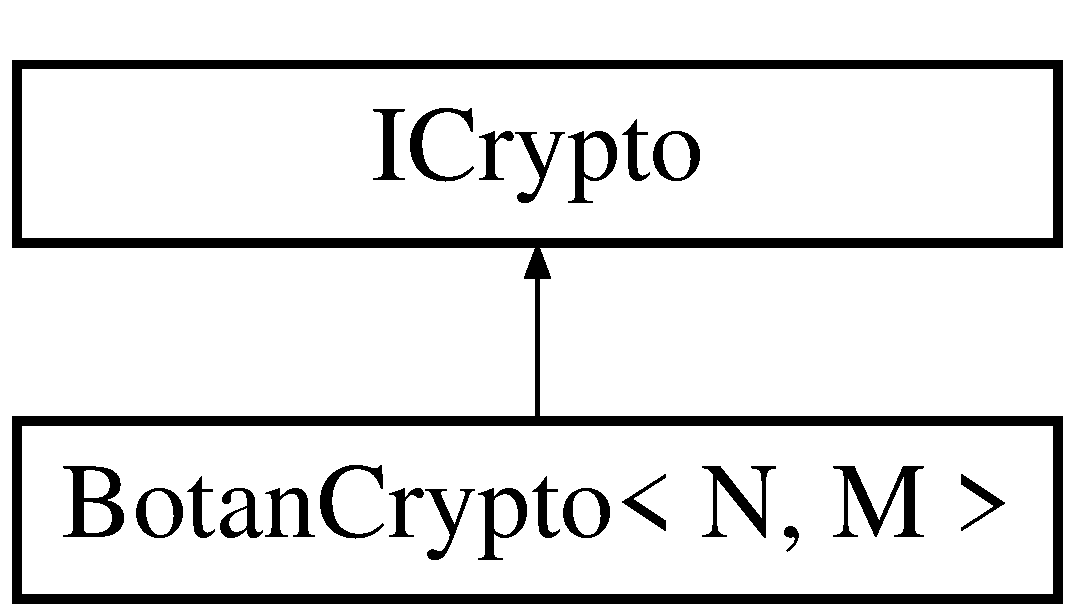
\includegraphics[height=2.000000cm]{classefb_1_1BotanCrypto}
\end{center}
\end{figure}
\subsection*{Public Member Functions}
\begin{DoxyCompactItemize}
\item 
\hyperlink{classefb_1_1BotanCrypto_a0c0158c6ffe67cd6db789dd6a6c6cc17}{BotanCrypto} ()
\item 
unsigned int \hyperlink{classefb_1_1BotanCrypto_aaaaf0d310c60207d6c545ed3a8b72fcd}{calculateHeaderSize} (unsigned int numOfIds) const 
\item 
void \hyperlink{classefb_1_1BotanCrypto_ace3300e249bf4305ddffeee43c13d844}{encryptMessage} (std::vector$<$ \hyperlink{structefb_1_1FacebookId}{FacebookId} $>$ \&ids, std::vector$<$ \hyperlink{namespaceefb_a0c8186d9b9b7880309c27230bbb5e69d}{byte} $>$ \&data)
\item 
void \hyperlink{classefb_1_1BotanCrypto_acb98871622014be1ac47d2126c04d4de}{decryptMessage} (std::vector$<$ \hyperlink{namespaceefb_a0c8186d9b9b7880309c27230bbb5e69d}{byte} $>$ \&data)
\end{DoxyCompactItemize}
\subsection*{Private Member Functions}
\begin{DoxyCompactItemize}
\item 
void \hyperlink{classefb_1_1BotanCrypto_adb7dda4b7a25248c0a2ef2304f963799}{generateNewIv} ()
\item 
void \hyperlink{classefb_1_1BotanCrypto_a6dfd64b465fd521ebad9db4cad7ab2b7}{generateNewMessageKey} ()
\item 
void \hyperlink{classefb_1_1BotanCrypto_a157ac4e58784b83f91ff8cc8ad0e3707}{setIv} (std::string \&ivstr)
\item 
void \hyperlink{classefb_1_1BotanCrypto_a432078e20f50920790d0a36d74a6db39}{setMessageKey} (std::string \&keystr)
\item 
void \hyperlink{classefb_1_1BotanCrypto_a1eadc5a54ba4734a94ade3a8a1196161}{getIv} (std::vector$<$ \hyperlink{namespaceefb_a0c8186d9b9b7880309c27230bbb5e69d}{byte} $>$ \&data)
\item 
void \hyperlink{classefb_1_1BotanCrypto_a62b318991e2c89cf7ccadbb9b9be5899}{getCipheredMessageKey} (\hyperlink{structefb_1_1FacebookId}{FacebookId} \&id, std::vector$<$ \hyperlink{namespaceefb_a0c8186d9b9b7880309c27230bbb5e69d}{byte} $>$ \&data)
\item 
void \hyperlink{classefb_1_1BotanCrypto_a77d2e662a29f4002bd2fb5fda7ec1753}{createCryptoHeader} (std::vector$<$ \hyperlink{structefb_1_1FacebookId}{FacebookId} $>$ \&ids, std::vector$<$ \hyperlink{namespaceefb_a0c8186d9b9b7880309c27230bbb5e69d}{byte} $>$ \&data)
\begin{DoxyCompactList}\small\item\em Create the crypto header using a new IV and message key. \item\end{DoxyCompactList}\item 
void \hyperlink{classefb_1_1BotanCrypto_af19ddf3f04af1a9bdc9ade40b259d75c}{parseCryptoHeader} (std::vector$<$ \hyperlink{namespaceefb_a0c8186d9b9b7880309c27230bbb5e69d}{byte} $>$ \&data)
\begin{DoxyCompactList}\small\item\em Attempty to parse a crypto header -\/ this will retrieve and set the message key and IV. \item\end{DoxyCompactList}\item 
unsigned int \hyperlink{classefb_1_1BotanCrypto_aeea9d6426438fd56e7ef699e9189993a}{retrieveHeaderSize} (std::vector$<$ \hyperlink{namespaceefb_a0c8186d9b9b7880309c27230bbb5e69d}{byte} $>$ \&data) const 
\begin{DoxyCompactList}\small\item\em Get the header size. \item\end{DoxyCompactList}\end{DoxyCompactItemize}
\subsection*{Private Attributes}
\begin{DoxyCompactItemize}
\item 
Botan::LibraryInitializer \hyperlink{classefb_1_1BotanCrypto_a8268da23ee821c4de9e701f6cfb8f97b}{init}
\begin{DoxyCompactList}\small\item\em Botan library members. \item\end{DoxyCompactList}\item 
Botan::AutoSeeded\_\-RNG \hyperlink{classefb_1_1BotanCrypto_af0dc1f5b610b421b2953da670c1df0ab}{rng}
\item 
Botan::SymmetricKey \hyperlink{classefb_1_1BotanCrypto_ad10c9baa2a09c7cbc7913d36a9f9afc1}{key}
\item 
Botan::InitializationVector \hyperlink{classefb_1_1BotanCrypto_a2bf475fe01a413ade4ab3e1cb26b8435}{iv}
\end{DoxyCompactItemize}


\subsection{Detailed Description}
\subsubsection*{template$<$int N, int M$>$ class efb::BotanCrypto$<$ N, M $>$}

Botan cryptography class using N-\/byte AES and M-\/byte RSA. This class uses the Botan cryptography library to perform encryption and decryption in place. AES and RSA are the symmetric and asymmetric (respectively) schemes employed. The template variables $<$N,M$>$ determine the key lengths. The header consists of two length bytes specifying the number of recipients, the message IV in plaintext, and a sequence of (Facebook ID, message-\/key) pairs. Each message-\/key is encrypted under the public key of the Facebook ID it is paired with. 

\subsection{Constructor \& Destructor Documentation}
\hypertarget{classefb_1_1BotanCrypto_a0c0158c6ffe67cd6db789dd6a6c6cc17}{
\index{efb::BotanCrypto@{efb::BotanCrypto}!BotanCrypto@{BotanCrypto}}
\index{BotanCrypto@{BotanCrypto}!efb::BotanCrypto@{efb::BotanCrypto}}
\subsubsection[{BotanCrypto}]{\setlength{\rightskip}{0pt plus 5cm}{\bf BotanCrypto} (
\begin{DoxyParamCaption}
{}
\end{DoxyParamCaption}
)}}
\label{classefb_1_1BotanCrypto_a0c0158c6ffe67cd6db789dd6a6c6cc17}


\subsection{Member Function Documentation}
\hypertarget{classefb_1_1BotanCrypto_adb7dda4b7a25248c0a2ef2304f963799}{
\index{efb::BotanCrypto@{efb::BotanCrypto}!generateNewIv@{generateNewIv}}
\index{generateNewIv@{generateNewIv}!efb::BotanCrypto@{efb::BotanCrypto}}
\subsubsection[{generateNewIv}]{\setlength{\rightskip}{0pt plus 5cm}void generateNewIv (
\begin{DoxyParamCaption}
{}
\end{DoxyParamCaption}
)\hspace{0.3cm}{\ttfamily  \mbox{[}private\mbox{]}}}}
\label{classefb_1_1BotanCrypto_adb7dda4b7a25248c0a2ef2304f963799}
\hypertarget{classefb_1_1BotanCrypto_a6dfd64b465fd521ebad9db4cad7ab2b7}{
\index{efb::BotanCrypto@{efb::BotanCrypto}!generateNewMessageKey@{generateNewMessageKey}}
\index{generateNewMessageKey@{generateNewMessageKey}!efb::BotanCrypto@{efb::BotanCrypto}}
\subsubsection[{generateNewMessageKey}]{\setlength{\rightskip}{0pt plus 5cm}void generateNewMessageKey (
\begin{DoxyParamCaption}
{}
\end{DoxyParamCaption}
)\hspace{0.3cm}{\ttfamily  \mbox{[}private\mbox{]}}}}
\label{classefb_1_1BotanCrypto_a6dfd64b465fd521ebad9db4cad7ab2b7}
\hypertarget{classefb_1_1BotanCrypto_a157ac4e58784b83f91ff8cc8ad0e3707}{
\index{efb::BotanCrypto@{efb::BotanCrypto}!setIv@{setIv}}
\index{setIv@{setIv}!efb::BotanCrypto@{efb::BotanCrypto}}
\subsubsection[{setIv}]{\setlength{\rightskip}{0pt plus 5cm}void setIv (
\begin{DoxyParamCaption}
\item[{std::string \&}]{ ivstr}
\end{DoxyParamCaption}
)\hspace{0.3cm}{\ttfamily  \mbox{[}private\mbox{]}}}}
\label{classefb_1_1BotanCrypto_a157ac4e58784b83f91ff8cc8ad0e3707}
\hypertarget{classefb_1_1BotanCrypto_a432078e20f50920790d0a36d74a6db39}{
\index{efb::BotanCrypto@{efb::BotanCrypto}!setMessageKey@{setMessageKey}}
\index{setMessageKey@{setMessageKey}!efb::BotanCrypto@{efb::BotanCrypto}}
\subsubsection[{setMessageKey}]{\setlength{\rightskip}{0pt plus 5cm}void setMessageKey (
\begin{DoxyParamCaption}
\item[{std::string \&}]{ keystr}
\end{DoxyParamCaption}
)\hspace{0.3cm}{\ttfamily  \mbox{[}private\mbox{]}}}}
\label{classefb_1_1BotanCrypto_a432078e20f50920790d0a36d74a6db39}
\hypertarget{classefb_1_1BotanCrypto_a1eadc5a54ba4734a94ade3a8a1196161}{
\index{efb::BotanCrypto@{efb::BotanCrypto}!getIv@{getIv}}
\index{getIv@{getIv}!efb::BotanCrypto@{efb::BotanCrypto}}
\subsubsection[{getIv}]{\setlength{\rightskip}{0pt plus 5cm}void getIv (
\begin{DoxyParamCaption}
\item[{std::vector$<$ {\bf byte} $>$ \&}]{ data}
\end{DoxyParamCaption}
)\hspace{0.3cm}{\ttfamily  \mbox{[}private\mbox{]}}}}
\label{classefb_1_1BotanCrypto_a1eadc5a54ba4734a94ade3a8a1196161}
\hypertarget{classefb_1_1BotanCrypto_a62b318991e2c89cf7ccadbb9b9be5899}{
\index{efb::BotanCrypto@{efb::BotanCrypto}!getCipheredMessageKey@{getCipheredMessageKey}}
\index{getCipheredMessageKey@{getCipheredMessageKey}!efb::BotanCrypto@{efb::BotanCrypto}}
\subsubsection[{getCipheredMessageKey}]{\setlength{\rightskip}{0pt plus 5cm}void getCipheredMessageKey (
\begin{DoxyParamCaption}
\item[{{\bf FacebookId} \&}]{ id, }
\item[{std::vector$<$ {\bf byte} $>$ \&}]{ data}
\end{DoxyParamCaption}
)\hspace{0.3cm}{\ttfamily  \mbox{[}private\mbox{]}}}}
\label{classefb_1_1BotanCrypto_a62b318991e2c89cf7ccadbb9b9be5899}
\hypertarget{classefb_1_1BotanCrypto_a77d2e662a29f4002bd2fb5fda7ec1753}{
\index{efb::BotanCrypto@{efb::BotanCrypto}!createCryptoHeader@{createCryptoHeader}}
\index{createCryptoHeader@{createCryptoHeader}!efb::BotanCrypto@{efb::BotanCrypto}}
\subsubsection[{createCryptoHeader}]{\setlength{\rightskip}{0pt plus 5cm}void createCryptoHeader (
\begin{DoxyParamCaption}
\item[{std::vector$<$ {\bf FacebookId} $>$ \&}]{ ids, }
\item[{std::vector$<$ {\bf byte} $>$ \&}]{ data}
\end{DoxyParamCaption}
)\hspace{0.3cm}{\ttfamily  \mbox{[}private\mbox{]}}}}
\label{classefb_1_1BotanCrypto_a77d2e662a29f4002bd2fb5fda7ec1753}


Create the crypto header using a new IV and message key. 

\hypertarget{classefb_1_1BotanCrypto_af19ddf3f04af1a9bdc9ade40b259d75c}{
\index{efb::BotanCrypto@{efb::BotanCrypto}!parseCryptoHeader@{parseCryptoHeader}}
\index{parseCryptoHeader@{parseCryptoHeader}!efb::BotanCrypto@{efb::BotanCrypto}}
\subsubsection[{parseCryptoHeader}]{\setlength{\rightskip}{0pt plus 5cm}void parseCryptoHeader (
\begin{DoxyParamCaption}
\item[{std::vector$<$ {\bf byte} $>$ \&}]{ data}
\end{DoxyParamCaption}
)\hspace{0.3cm}{\ttfamily  \mbox{[}private\mbox{]}}}}
\label{classefb_1_1BotanCrypto_af19ddf3f04af1a9bdc9ade40b259d75c}


Attempty to parse a crypto header -\/ this will retrieve and set the message key and IV. 

\hypertarget{classefb_1_1BotanCrypto_aeea9d6426438fd56e7ef699e9189993a}{
\index{efb::BotanCrypto@{efb::BotanCrypto}!retrieveHeaderSize@{retrieveHeaderSize}}
\index{retrieveHeaderSize@{retrieveHeaderSize}!efb::BotanCrypto@{efb::BotanCrypto}}
\subsubsection[{retrieveHeaderSize}]{\setlength{\rightskip}{0pt plus 5cm}unsigned int retrieveHeaderSize (
\begin{DoxyParamCaption}
\item[{std::vector$<$ {\bf byte} $>$ \&}]{ data}
\end{DoxyParamCaption}
) const\hspace{0.3cm}{\ttfamily  \mbox{[}private\mbox{]}}}}
\label{classefb_1_1BotanCrypto_aeea9d6426438fd56e7ef699e9189993a}


Get the header size. 

\hypertarget{classefb_1_1BotanCrypto_aaaaf0d310c60207d6c545ed3a8b72fcd}{
\index{efb::BotanCrypto@{efb::BotanCrypto}!calculateHeaderSize@{calculateHeaderSize}}
\index{calculateHeaderSize@{calculateHeaderSize}!efb::BotanCrypto@{efb::BotanCrypto}}
\subsubsection[{calculateHeaderSize}]{\setlength{\rightskip}{0pt plus 5cm}unsigned int calculateHeaderSize (
\begin{DoxyParamCaption}
\item[{unsigned int}]{ numOfIds}
\end{DoxyParamCaption}
) const\hspace{0.3cm}{\ttfamily  \mbox{[}virtual\mbox{]}}}}
\label{classefb_1_1BotanCrypto_aaaaf0d310c60207d6c545ed3a8b72fcd}


Implements \hyperlink{classefb_1_1ICrypto_a1d1ef41942f8d5c114ffd8180fbe547f}{ICrypto}.

\hypertarget{classefb_1_1BotanCrypto_ace3300e249bf4305ddffeee43c13d844}{
\index{efb::BotanCrypto@{efb::BotanCrypto}!encryptMessage@{encryptMessage}}
\index{encryptMessage@{encryptMessage}!efb::BotanCrypto@{efb::BotanCrypto}}
\subsubsection[{encryptMessage}]{\setlength{\rightskip}{0pt plus 5cm}void encryptMessage (
\begin{DoxyParamCaption}
\item[{std::vector$<$ {\bf FacebookId} $>$ \&}]{ ids, }
\item[{std::vector$<$ {\bf byte} $>$ \&}]{ data}
\end{DoxyParamCaption}
)\hspace{0.3cm}{\ttfamily  \mbox{[}virtual\mbox{]}}}}
\label{classefb_1_1BotanCrypto_ace3300e249bf4305ddffeee43c13d844}


Implements \hyperlink{classefb_1_1ICrypto_a258cb59b2942fbac3615b14207dbdf78}{ICrypto}.

\hypertarget{classefb_1_1BotanCrypto_acb98871622014be1ac47d2126c04d4de}{
\index{efb::BotanCrypto@{efb::BotanCrypto}!decryptMessage@{decryptMessage}}
\index{decryptMessage@{decryptMessage}!efb::BotanCrypto@{efb::BotanCrypto}}
\subsubsection[{decryptMessage}]{\setlength{\rightskip}{0pt plus 5cm}void decryptMessage (
\begin{DoxyParamCaption}
\item[{std::vector$<$ {\bf byte} $>$ \&}]{ data}
\end{DoxyParamCaption}
)\hspace{0.3cm}{\ttfamily  \mbox{[}virtual\mbox{]}}}}
\label{classefb_1_1BotanCrypto_acb98871622014be1ac47d2126c04d4de}


Implements \hyperlink{classefb_1_1ICrypto_ac7d12b1021fd2f4bef93aac3169a35db}{ICrypto}.



\subsection{Member Data Documentation}
\hypertarget{classefb_1_1BotanCrypto_a8268da23ee821c4de9e701f6cfb8f97b}{
\index{efb::BotanCrypto@{efb::BotanCrypto}!init@{init}}
\index{init@{init}!efb::BotanCrypto@{efb::BotanCrypto}}
\subsubsection[{init}]{\setlength{\rightskip}{0pt plus 5cm}Botan::LibraryInitializer {\bf init}\hspace{0.3cm}{\ttfamily  \mbox{[}private\mbox{]}}}}
\label{classefb_1_1BotanCrypto_a8268da23ee821c4de9e701f6cfb8f97b}


Botan library members. 

\hypertarget{classefb_1_1BotanCrypto_af0dc1f5b610b421b2953da670c1df0ab}{
\index{efb::BotanCrypto@{efb::BotanCrypto}!rng@{rng}}
\index{rng@{rng}!efb::BotanCrypto@{efb::BotanCrypto}}
\subsubsection[{rng}]{\setlength{\rightskip}{0pt plus 5cm}Botan::AutoSeeded\_\-RNG {\bf rng}\hspace{0.3cm}{\ttfamily  \mbox{[}private\mbox{]}}}}
\label{classefb_1_1BotanCrypto_af0dc1f5b610b421b2953da670c1df0ab}
\hypertarget{classefb_1_1BotanCrypto_ad10c9baa2a09c7cbc7913d36a9f9afc1}{
\index{efb::BotanCrypto@{efb::BotanCrypto}!key@{key}}
\index{key@{key}!efb::BotanCrypto@{efb::BotanCrypto}}
\subsubsection[{key}]{\setlength{\rightskip}{0pt plus 5cm}Botan::SymmetricKey {\bf key}\hspace{0.3cm}{\ttfamily  \mbox{[}private\mbox{]}}}}
\label{classefb_1_1BotanCrypto_ad10c9baa2a09c7cbc7913d36a9f9afc1}
\hypertarget{classefb_1_1BotanCrypto_a2bf475fe01a413ade4ab3e1cb26b8435}{
\index{efb::BotanCrypto@{efb::BotanCrypto}!iv@{iv}}
\index{iv@{iv}!efb::BotanCrypto@{efb::BotanCrypto}}
\subsubsection[{iv}]{\setlength{\rightskip}{0pt plus 5cm}Botan::InitializationVector {\bf iv}\hspace{0.3cm}{\ttfamily  \mbox{[}private\mbox{]}}}}
\label{classefb_1_1BotanCrypto_a2bf475fe01a413ade4ab3e1cb26b8435}

\hypertarget{classefb_1_1Core}{
\section{Core Class Reference}
\label{classefb_1_1Core}\index{efb::Core@{efb::Core}}
}
Inheritance diagram for Core:\begin{figure}[H]
\begin{center}
\leavevmode
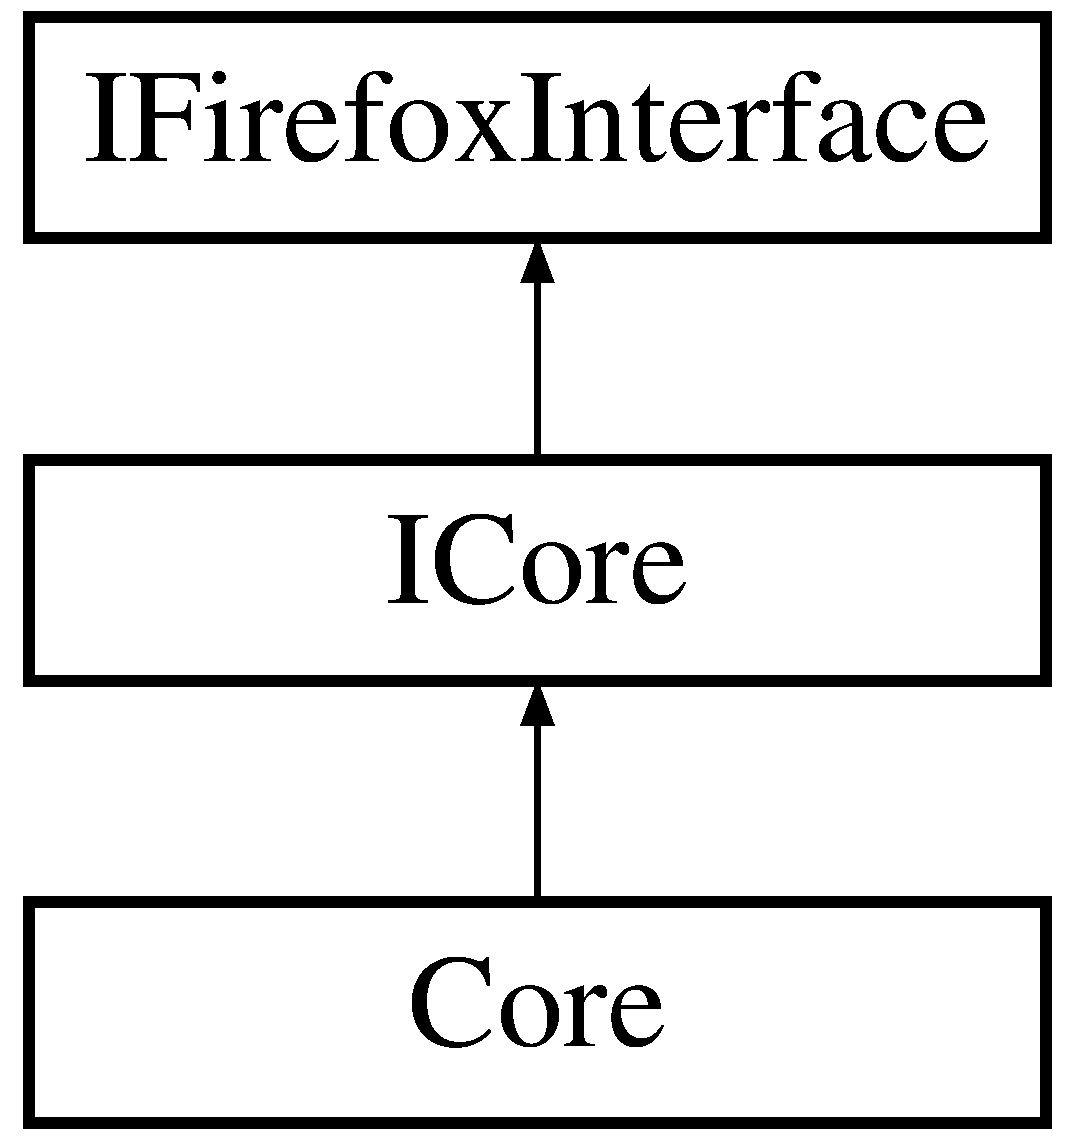
\includegraphics[height=3.000000cm]{classefb_1_1Core}
\end{center}
\end{figure}

\hypertarget{structefb_1_1FacebookId}{
\section{FacebookId Struct Reference}
\label{structefb_1_1FacebookId}\index{efb::FacebookId@{efb::FacebookId}}
}
\subsection*{Public Attributes}
\begin{DoxyCompactItemize}
\item 
unsigned int \hyperlink{structefb_1_1FacebookId_a8b464957786ffe5a3406a4060f0da97f}{hi}
\item 
unsigned int \hyperlink{structefb_1_1FacebookId_af0c1fc19ce0b4c36f5b6a41b90012403}{lo}
\end{DoxyCompactItemize}


\subsection{Member Data Documentation}
\hypertarget{structefb_1_1FacebookId_a8b464957786ffe5a3406a4060f0da97f}{
\index{efb::FacebookId@{efb::FacebookId}!hi@{hi}}
\index{hi@{hi}!efb::FacebookId@{efb::FacebookId}}
\subsubsection[{hi}]{\setlength{\rightskip}{0pt plus 5cm}unsigned int {\bf hi}}}
\label{structefb_1_1FacebookId_a8b464957786ffe5a3406a4060f0da97f}
\hypertarget{structefb_1_1FacebookId_af0c1fc19ce0b4c36f5b6a41b90012403}{
\index{efb::FacebookId@{efb::FacebookId}!lo@{lo}}
\index{lo@{lo}!efb::FacebookId@{efb::FacebookId}}
\subsubsection[{lo}]{\setlength{\rightskip}{0pt plus 5cm}unsigned int {\bf lo}}}
\label{structefb_1_1FacebookId_af0c1fc19ce0b4c36f5b6a41b90012403}

\hypertarget{classefb_1_1HaarConduitImage}{
\section{HaarConduitImage Class Reference}
\label{classefb_1_1HaarConduitImage}\index{efb::HaarConduitImage@{efb::HaarConduitImage}}
}
Inheritance diagram for HaarConduitImage:\begin{figure}[H]
\begin{center}
\leavevmode
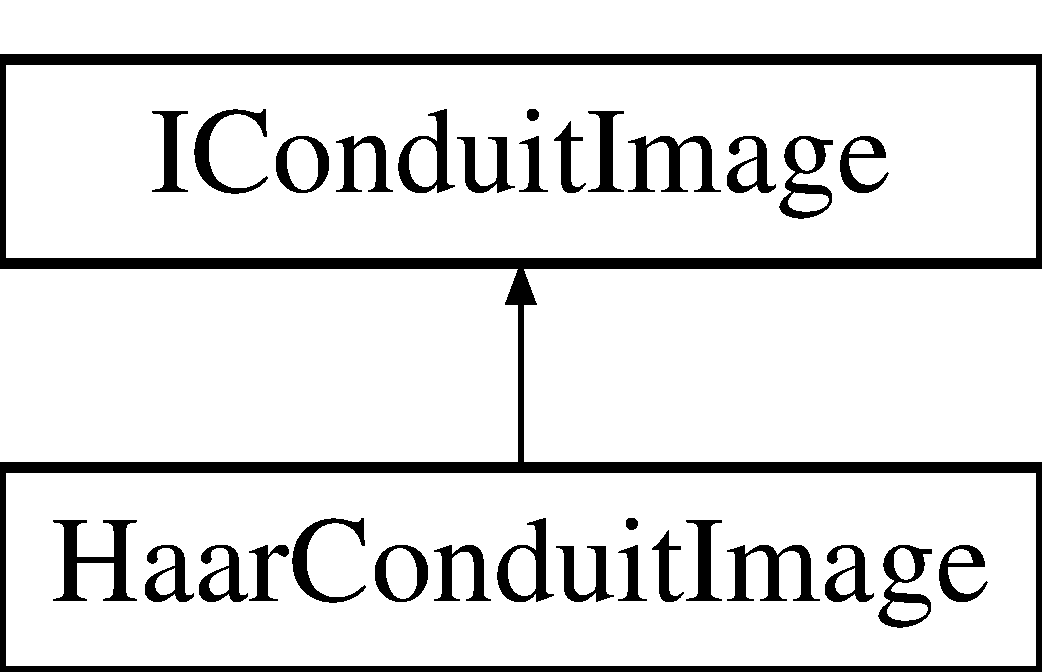
\includegraphics[height=2.000000cm]{classefb_1_1HaarConduitImage}
\end{center}
\end{figure}

\hypertarget{classefb_1_1IConduitImage}{
\section{IConduitImage Class Reference}
\label{classefb_1_1IConduitImage}\index{efb::IConduitImage@{efb::IConduitImage}}
}


Abstract class defining a conduit image, with functionality for implanting and extracting data.  


Inheritance diagram for IConduitImage:\begin{figure}[H]
\begin{center}
\leavevmode
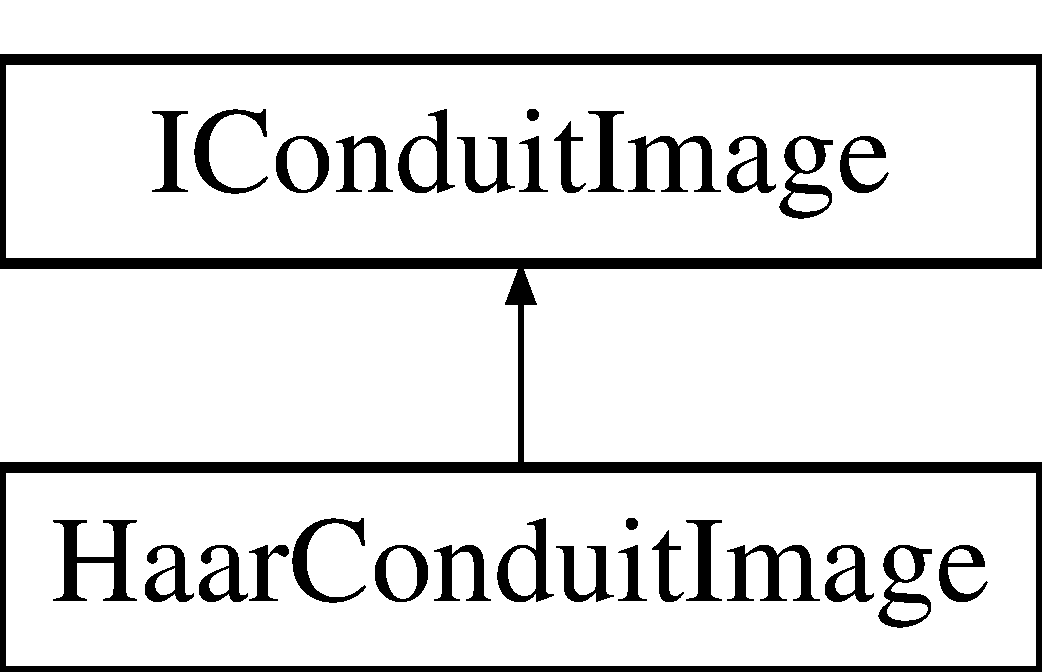
\includegraphics[height=2.000000cm]{classefb_1_1IConduitImage}
\end{center}
\end{figure}
\subsection*{Public Member Functions}
\begin{DoxyCompactItemize}
\item 
virtual unsigned int \hyperlink{classefb_1_1IConduitImage_adf25b030496042f8e063ad54806fcf9d}{getMaxData} ()=0
\begin{DoxyCompactList}\small\item\em Get the maximum ammount of data that can be stored in this implementation. \item\end{DoxyCompactList}\item 
virtual unsigned short \hyperlink{classefb_1_1IConduitImage_af4c6699ceacada4b0222ad4f1d1c384d}{readSize} ()=0
\begin{DoxyCompactList}\small\item\em Check how much data (if any) is stored in the current image. \item\end{DoxyCompactList}\item 
virtual void \hyperlink{classefb_1_1IConduitImage_aead78fe96a2ec4e676c7aaf018427671}{implantData} (std::vector$<$ char $>$ \&data)=0
\begin{DoxyCompactList}\small\item\em Implant data. \item\end{DoxyCompactList}\item 
virtual void \hyperlink{classefb_1_1IConduitImage_a920c1ba3f4f8d7531a8b6f8c8b38def6}{extractData} (std::vector$<$ char $>$ \&data)=0
\begin{DoxyCompactList}\small\item\em Extract data. \item\end{DoxyCompactList}\end{DoxyCompactItemize}


\subsection{Detailed Description}
Abstract class defining a conduit image, with functionality for implanting and extracting data. 

\subsection{Member Function Documentation}
\hypertarget{classefb_1_1IConduitImage_adf25b030496042f8e063ad54806fcf9d}{
\index{efb::IConduitImage@{efb::IConduitImage}!getMaxData@{getMaxData}}
\index{getMaxData@{getMaxData}!efb::IConduitImage@{efb::IConduitImage}}
\subsubsection[{getMaxData}]{\setlength{\rightskip}{0pt plus 5cm}virtual unsigned int getMaxData (
\begin{DoxyParamCaption}
{}
\end{DoxyParamCaption}
)\hspace{0.3cm}{\ttfamily  \mbox{[}pure virtual\mbox{]}}}}
\label{classefb_1_1IConduitImage_adf25b030496042f8e063ad54806fcf9d}


Get the maximum ammount of data that can be stored in this implementation. 

\hypertarget{classefb_1_1IConduitImage_af4c6699ceacada4b0222ad4f1d1c384d}{
\index{efb::IConduitImage@{efb::IConduitImage}!readSize@{readSize}}
\index{readSize@{readSize}!efb::IConduitImage@{efb::IConduitImage}}
\subsubsection[{readSize}]{\setlength{\rightskip}{0pt plus 5cm}virtual unsigned short readSize (
\begin{DoxyParamCaption}
{}
\end{DoxyParamCaption}
)\hspace{0.3cm}{\ttfamily  \mbox{[}pure virtual\mbox{]}}}}
\label{classefb_1_1IConduitImage_af4c6699ceacada4b0222ad4f1d1c384d}


Check how much data (if any) is stored in the current image. 



Implemented in \hyperlink{classefb_1_1HaarConduitImage_a5e272ba12218188cba439255dea9df40}{HaarConduitImage}.

\hypertarget{classefb_1_1IConduitImage_aead78fe96a2ec4e676c7aaf018427671}{
\index{efb::IConduitImage@{efb::IConduitImage}!implantData@{implantData}}
\index{implantData@{implantData}!efb::IConduitImage@{efb::IConduitImage}}
\subsubsection[{implantData}]{\setlength{\rightskip}{0pt plus 5cm}virtual void implantData (
\begin{DoxyParamCaption}
\item[{std::vector$<$ char $>$ \&}]{ data}
\end{DoxyParamCaption}
)\hspace{0.3cm}{\ttfamily  \mbox{[}pure virtual\mbox{]}}}}
\label{classefb_1_1IConduitImage_aead78fe96a2ec4e676c7aaf018427671}


Implant data. 



Implemented in \hyperlink{classefb_1_1HaarConduitImage_a722f5510d5b87afd72222afed3f77d34}{HaarConduitImage}.

\hypertarget{classefb_1_1IConduitImage_a920c1ba3f4f8d7531a8b6f8c8b38def6}{
\index{efb::IConduitImage@{efb::IConduitImage}!extractData@{extractData}}
\index{extractData@{extractData}!efb::IConduitImage@{efb::IConduitImage}}
\subsubsection[{extractData}]{\setlength{\rightskip}{0pt plus 5cm}virtual void extractData (
\begin{DoxyParamCaption}
\item[{std::vector$<$ char $>$ \&}]{ data}
\end{DoxyParamCaption}
)\hspace{0.3cm}{\ttfamily  \mbox{[}pure virtual\mbox{]}}}}
\label{classefb_1_1IConduitImage_a920c1ba3f4f8d7531a8b6f8c8b38def6}


Extract data. 



Implemented in \hyperlink{classefb_1_1HaarConduitImage_a34b2b3ff92ddfea24ccd0c1b6786152c}{HaarConduitImage}.


\hypertarget{classefb_1_1ICore}{
\section{ICore Class Reference}
\label{classefb_1_1ICore}\index{efb::ICore@{efb::ICore}}
}


\hyperlink{classefb_1_1Core}{Core} library class.  


Inheritance diagram for ICore:\begin{figure}[H]
\begin{center}
\leavevmode
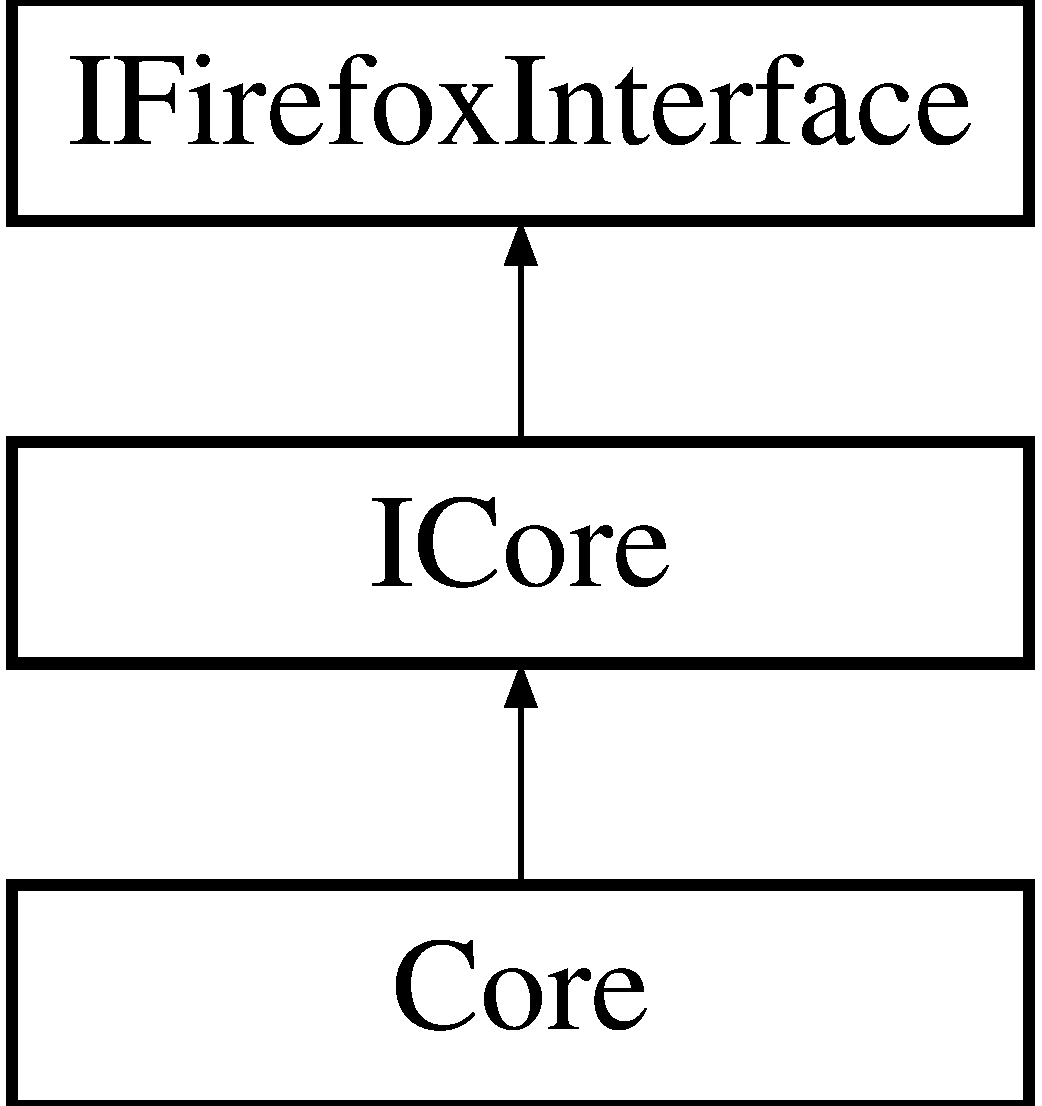
\includegraphics[height=3.000000cm]{classefb_1_1ICore}
\end{center}
\end{figure}
\subsection*{Private Member Functions}
\begin{DoxyCompactItemize}
\item 
void \hyperlink{classefb_1_1ICore_a758885d8fdb1b308587b2500df48b8ac}{init\_\-crypto} ()
\begin{DoxyCompactList}\small\item\em Initialiser for the cryptograhic library code. \item\end{DoxyCompactList}\item 
void \hyperlink{classefb_1_1ICore_a0b17fb5c4682b0e0a3aa266596759368}{init\_\-fec} ()
\begin{DoxyCompactList}\small\item\em Initialiser for the forward error correction library code. \item\end{DoxyCompactList}\item 
virtual \hyperlink{classefb_1_1IConduitImage}{IConduitImage} \& \hyperlink{classefb_1_1ICore_affa3abf2e0b92c8710a31cec5184e893}{create\_\-IConduitImage} ()=0
\begin{DoxyCompactList}\small\item\em Abstract factory pattern object creater. \item\end{DoxyCompactList}\item 
virtual \hyperlink{classefb_1_1ICrypto}{ICrypto} \& \hyperlink{classefb_1_1ICore_a4c27ca4eb5d68a4b509c74572a3b2d48}{create\_\-ICrypto} ()=0
\begin{DoxyCompactList}\small\item\em Abstract factory pattern object creater. \item\end{DoxyCompactList}\item 
virtual \hyperlink{classefb_1_1IFec}{IFec} \& \hyperlink{classefb_1_1ICore_a0f65d448a5b036921f1ddb9c00f7f5e2}{create\_\-IFec} ()=0
\begin{DoxyCompactList}\small\item\em Abstract factory pattern object creater. \item\end{DoxyCompactList}\end{DoxyCompactItemize}
\subsection*{Private Attributes}
\begin{DoxyCompactItemize}
\item 
\hyperlink{classefb_1_1ICrypto}{ICrypto} $\ast$ \hyperlink{classefb_1_1ICore_aa702cd793e531eb1c92bbefd55ff55f8}{crypto}
\begin{DoxyCompactList}\small\item\em Instance of the cryptographic library code. \item\end{DoxyCompactList}\item 
\hyperlink{classefb_1_1IFec}{IFec} $\ast$ \hyperlink{classefb_1_1ICore_affa4ef963558c4749811b1b9eefb2898}{fec}
\begin{DoxyCompactList}\small\item\em Instance of the forward error correction library code. \item\end{DoxyCompactList}\end{DoxyCompactItemize}


\subsection{Detailed Description}
\hyperlink{classefb_1_1Core}{Core} library class. This is the main library class. Other library components (cryptography and error correction) are grouped into further classes and instantiated as attribute members. 

\subsection{Member Function Documentation}
\hypertarget{classefb_1_1ICore_a758885d8fdb1b308587b2500df48b8ac}{
\index{efb::ICore@{efb::ICore}!init\_\-crypto@{init\_\-crypto}}
\index{init\_\-crypto@{init\_\-crypto}!efb::ICore@{efb::ICore}}
\subsubsection[{init\_\-crypto}]{\setlength{\rightskip}{0pt plus 5cm}void init\_\-crypto (
\begin{DoxyParamCaption}
{}
\end{DoxyParamCaption}
)\hspace{0.3cm}{\ttfamily  \mbox{[}private\mbox{]}}}}
\label{classefb_1_1ICore_a758885d8fdb1b308587b2500df48b8ac}


Initialiser for the cryptograhic library code. 

\hypertarget{classefb_1_1ICore_a0b17fb5c4682b0e0a3aa266596759368}{
\index{efb::ICore@{efb::ICore}!init\_\-fec@{init\_\-fec}}
\index{init\_\-fec@{init\_\-fec}!efb::ICore@{efb::ICore}}
\subsubsection[{init\_\-fec}]{\setlength{\rightskip}{0pt plus 5cm}void init\_\-fec (
\begin{DoxyParamCaption}
{}
\end{DoxyParamCaption}
)\hspace{0.3cm}{\ttfamily  \mbox{[}private\mbox{]}}}}
\label{classefb_1_1ICore_a0b17fb5c4682b0e0a3aa266596759368}


Initialiser for the forward error correction library code. 

\hypertarget{classefb_1_1ICore_affa3abf2e0b92c8710a31cec5184e893}{
\index{efb::ICore@{efb::ICore}!create\_\-IConduitImage@{create\_\-IConduitImage}}
\index{create\_\-IConduitImage@{create\_\-IConduitImage}!efb::ICore@{efb::ICore}}
\subsubsection[{create\_\-IConduitImage}]{\setlength{\rightskip}{0pt plus 5cm}virtual {\bf IConduitImage}\& create\_\-IConduitImage (
\begin{DoxyParamCaption}
{}
\end{DoxyParamCaption}
)\hspace{0.3cm}{\ttfamily  \mbox{[}private, pure virtual\mbox{]}}}}
\label{classefb_1_1ICore_affa3abf2e0b92c8710a31cec5184e893}


Abstract factory pattern object creater. 

\hypertarget{classefb_1_1ICore_a4c27ca4eb5d68a4b509c74572a3b2d48}{
\index{efb::ICore@{efb::ICore}!create\_\-ICrypto@{create\_\-ICrypto}}
\index{create\_\-ICrypto@{create\_\-ICrypto}!efb::ICore@{efb::ICore}}
\subsubsection[{create\_\-ICrypto}]{\setlength{\rightskip}{0pt plus 5cm}virtual {\bf ICrypto}\& create\_\-ICrypto (
\begin{DoxyParamCaption}
{}
\end{DoxyParamCaption}
)\hspace{0.3cm}{\ttfamily  \mbox{[}private, pure virtual\mbox{]}}}}
\label{classefb_1_1ICore_a4c27ca4eb5d68a4b509c74572a3b2d48}


Abstract factory pattern object creater. 

\hypertarget{classefb_1_1ICore_a0f65d448a5b036921f1ddb9c00f7f5e2}{
\index{efb::ICore@{efb::ICore}!create\_\-IFec@{create\_\-IFec}}
\index{create\_\-IFec@{create\_\-IFec}!efb::ICore@{efb::ICore}}
\subsubsection[{create\_\-IFec}]{\setlength{\rightskip}{0pt plus 5cm}virtual {\bf IFec}\& create\_\-IFec (
\begin{DoxyParamCaption}
{}
\end{DoxyParamCaption}
)\hspace{0.3cm}{\ttfamily  \mbox{[}private, pure virtual\mbox{]}}}}
\label{classefb_1_1ICore_a0f65d448a5b036921f1ddb9c00f7f5e2}


Abstract factory pattern object creater. 



\subsection{Member Data Documentation}
\hypertarget{classefb_1_1ICore_aa702cd793e531eb1c92bbefd55ff55f8}{
\index{efb::ICore@{efb::ICore}!crypto@{crypto}}
\index{crypto@{crypto}!efb::ICore@{efb::ICore}}
\subsubsection[{crypto}]{\setlength{\rightskip}{0pt plus 5cm}{\bf ICrypto}$\ast$ {\bf crypto}\hspace{0.3cm}{\ttfamily  \mbox{[}private\mbox{]}}}}
\label{classefb_1_1ICore_aa702cd793e531eb1c92bbefd55ff55f8}


Instance of the cryptographic library code. 

\hypertarget{classefb_1_1ICore_affa4ef963558c4749811b1b9eefb2898}{
\index{efb::ICore@{efb::ICore}!fec@{fec}}
\index{fec@{fec}!efb::ICore@{efb::ICore}}
\subsubsection[{fec}]{\setlength{\rightskip}{0pt plus 5cm}{\bf IFec}$\ast$ {\bf fec}\hspace{0.3cm}{\ttfamily  \mbox{[}private\mbox{]}}}}
\label{classefb_1_1ICore_affa4ef963558c4749811b1b9eefb2898}


Instance of the forward error correction library code. 


\hypertarget{classefb_1_1ICrypto}{
\section{ICrypto Class Reference}
\label{classefb_1_1ICrypto}\index{efb::ICrypto@{efb::ICrypto}}
}


Abstract class definining the interface for the cryptographic algorithms.  


Inheritance diagram for ICrypto:\begin{figure}[H]
\begin{center}
\leavevmode
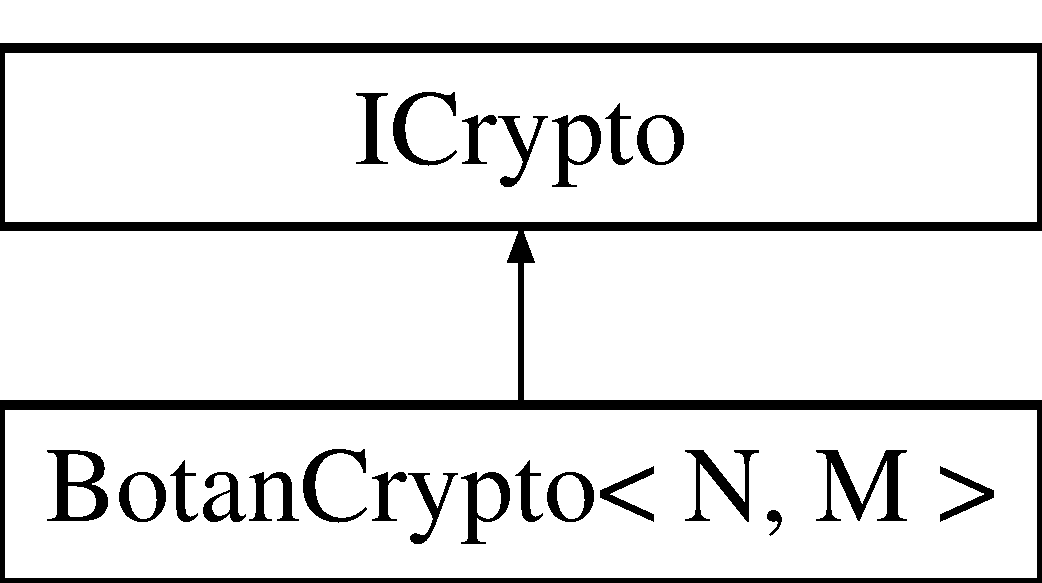
\includegraphics[height=2.000000cm]{classefb_1_1ICrypto}
\end{center}
\end{figure}
\subsection*{Public Member Functions}
\begin{DoxyCompactItemize}
\item 
virtual unsigned int \hyperlink{classefb_1_1ICrypto_a1d1ef41942f8d5c114ffd8180fbe547f}{calculateHeaderSize} (unsigned int numOfIds) const =0
\begin{DoxyCompactList}\small\item\em Returns the predicted header size so we can leave room before encryption. \item\end{DoxyCompactList}\item 
virtual void \hyperlink{classefb_1_1ICrypto_a258cb59b2942fbac3615b14207dbdf78}{encryptMessage} (std::vector$<$ \hyperlink{structefb_1_1FacebookId}{FacebookId} $>$ \&ids, std::vector$<$ \hyperlink{namespaceefb_a0c8186d9b9b7880309c27230bbb5e69d}{byte} $>$ \&data)=0
\begin{DoxyCompactList}\small\item\em Writes header and encrypts message. Assumes there is a header-\/size offset before data bytes begin. \item\end{DoxyCompactList}\item 
virtual void \hyperlink{classefb_1_1ICrypto_ac7d12b1021fd2f4bef93aac3169a35db}{decryptMessage} (std::vector$<$ \hyperlink{namespaceefb_a0c8186d9b9b7880309c27230bbb5e69d}{byte} $>$ \&data)=0
\begin{DoxyCompactList}\small\item\em Parses any data header and attempts to decrypt the data. \item\end{DoxyCompactList}\end{DoxyCompactItemize}


\subsection{Detailed Description}
Abstract class definining the interface for the cryptographic algorithms. 

\subsection{Member Function Documentation}
\hypertarget{classefb_1_1ICrypto_a1d1ef41942f8d5c114ffd8180fbe547f}{
\index{efb::ICrypto@{efb::ICrypto}!calculateHeaderSize@{calculateHeaderSize}}
\index{calculateHeaderSize@{calculateHeaderSize}!efb::ICrypto@{efb::ICrypto}}
\subsubsection[{calculateHeaderSize}]{\setlength{\rightskip}{0pt plus 5cm}virtual unsigned int calculateHeaderSize (
\begin{DoxyParamCaption}
\item[{unsigned int}]{ numOfIds}
\end{DoxyParamCaption}
) const\hspace{0.3cm}{\ttfamily  \mbox{[}pure virtual\mbox{]}}}}
\label{classefb_1_1ICrypto_a1d1ef41942f8d5c114ffd8180fbe547f}


Returns the predicted header size so we can leave room before encryption. 



Implemented in \hyperlink{classefb_1_1BotanCrypto_aaaaf0d310c60207d6c545ed3a8b72fcd}{BotanCrypto$<$ N, M $>$}.

\hypertarget{classefb_1_1ICrypto_a258cb59b2942fbac3615b14207dbdf78}{
\index{efb::ICrypto@{efb::ICrypto}!encryptMessage@{encryptMessage}}
\index{encryptMessage@{encryptMessage}!efb::ICrypto@{efb::ICrypto}}
\subsubsection[{encryptMessage}]{\setlength{\rightskip}{0pt plus 5cm}virtual void encryptMessage (
\begin{DoxyParamCaption}
\item[{std::vector$<$ {\bf FacebookId} $>$ \&}]{ ids, }
\item[{std::vector$<$ {\bf byte} $>$ \&}]{ data}
\end{DoxyParamCaption}
)\hspace{0.3cm}{\ttfamily  \mbox{[}pure virtual\mbox{]}}}}
\label{classefb_1_1ICrypto_a258cb59b2942fbac3615b14207dbdf78}


Writes header and encrypts message. Assumes there is a header-\/size offset before data bytes begin. 



Implemented in \hyperlink{classefb_1_1BotanCrypto_ace3300e249bf4305ddffeee43c13d844}{BotanCrypto$<$ N, M $>$}.

\hypertarget{classefb_1_1ICrypto_ac7d12b1021fd2f4bef93aac3169a35db}{
\index{efb::ICrypto@{efb::ICrypto}!decryptMessage@{decryptMessage}}
\index{decryptMessage@{decryptMessage}!efb::ICrypto@{efb::ICrypto}}
\subsubsection[{decryptMessage}]{\setlength{\rightskip}{0pt plus 5cm}virtual void decryptMessage (
\begin{DoxyParamCaption}
\item[{std::vector$<$ {\bf byte} $>$ \&}]{ data}
\end{DoxyParamCaption}
)\hspace{0.3cm}{\ttfamily  \mbox{[}pure virtual\mbox{]}}}}
\label{classefb_1_1ICrypto_ac7d12b1021fd2f4bef93aac3169a35db}


Parses any data header and attempts to decrypt the data. 



Implemented in \hyperlink{classefb_1_1BotanCrypto_acb98871622014be1ac47d2126c04d4de}{BotanCrypto$<$ N, M $>$}.


\hypertarget{classefb_1_1IFec}{
\section{IFec Class Reference}
\label{classefb_1_1IFec}\index{efb::IFec@{efb::IFec}}
}


Abstract class definining the interface for the error correction algorithms.  


Inheritance diagram for IFec:\begin{figure}[H]
\begin{center}
\leavevmode
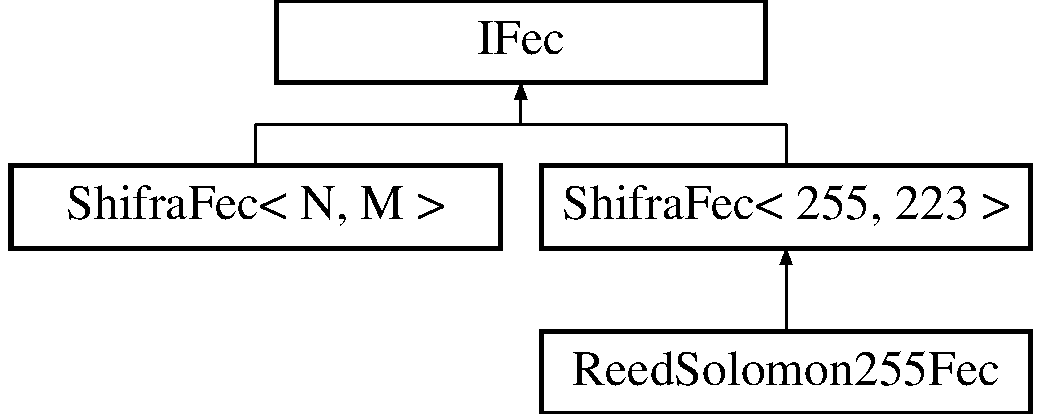
\includegraphics[height=3.000000cm]{classefb_1_1IFec}
\end{center}
\end{figure}
\subsection*{Public Member Functions}
\begin{DoxyCompactItemize}
\item 
virtual std::vector$<$ \hyperlink{namespaceefb_a0c8186d9b9b7880309c27230bbb5e69d}{byte} $>$ \& \hyperlink{classefb_1_1IFec_af8204657b9bd4cef16bff02d9e6256f8}{encode} (std::vector$<$ \hyperlink{namespaceefb_a0c8186d9b9b7880309c27230bbb5e69d}{byte} $>$ \&data)
\begin{DoxyCompactList}\small\item\em Encode data into a new vector. \item\end{DoxyCompactList}\item 
virtual std::vector$<$ \hyperlink{namespaceefb_a0c8186d9b9b7880309c27230bbb5e69d}{byte} $>$ \& \hyperlink{classefb_1_1IFec_ae214f6def8bf8f1b560b8f3bbdb5271b}{decode} (std::vector$<$ \hyperlink{namespaceefb_a0c8186d9b9b7880309c27230bbb5e69d}{byte} $>$ \&data)
\begin{DoxyCompactList}\small\item\em Decode (correct) data into a new vector. \item\end{DoxyCompactList}\end{DoxyCompactItemize}


\subsection{Detailed Description}
Abstract class definining the interface for the error correction algorithms. 

\subsection{Member Function Documentation}
\hypertarget{classefb_1_1IFec_af8204657b9bd4cef16bff02d9e6256f8}{
\index{efb::IFec@{efb::IFec}!encode@{encode}}
\index{encode@{encode}!efb::IFec@{efb::IFec}}
\subsubsection[{encode}]{\setlength{\rightskip}{0pt plus 5cm}virtual std::vector$<${\bf byte}$>$\& encode (
\begin{DoxyParamCaption}
\item[{std::vector$<$ {\bf byte} $>$ \&}]{ data}
\end{DoxyParamCaption}
)\hspace{0.3cm}{\ttfamily  \mbox{[}virtual\mbox{]}}}}
\label{classefb_1_1IFec_af8204657b9bd4cef16bff02d9e6256f8}


Encode data into a new vector. 

\hypertarget{classefb_1_1IFec_ae214f6def8bf8f1b560b8f3bbdb5271b}{
\index{efb::IFec@{efb::IFec}!decode@{decode}}
\index{decode@{decode}!efb::IFec@{efb::IFec}}
\subsubsection[{decode}]{\setlength{\rightskip}{0pt plus 5cm}virtual std::vector$<${\bf byte}$>$\& decode (
\begin{DoxyParamCaption}
\item[{std::vector$<$ {\bf byte} $>$ \&}]{ data}
\end{DoxyParamCaption}
)\hspace{0.3cm}{\ttfamily  \mbox{[}virtual\mbox{]}}}}
\label{classefb_1_1IFec_ae214f6def8bf8f1b560b8f3bbdb5271b}


Decode (correct) data into a new vector. 


\hypertarget{classefb_1_1IFirefoxInterface}{
\section{IFirefoxInterface Class Reference}
\label{classefb_1_1IFirefoxInterface}\index{efb::IFirefoxInterface@{efb::IFirefoxInterface}}
}


Firefox interface definition.  


Inheritance diagram for IFirefoxInterface:\begin{figure}[H]
\begin{center}
\leavevmode
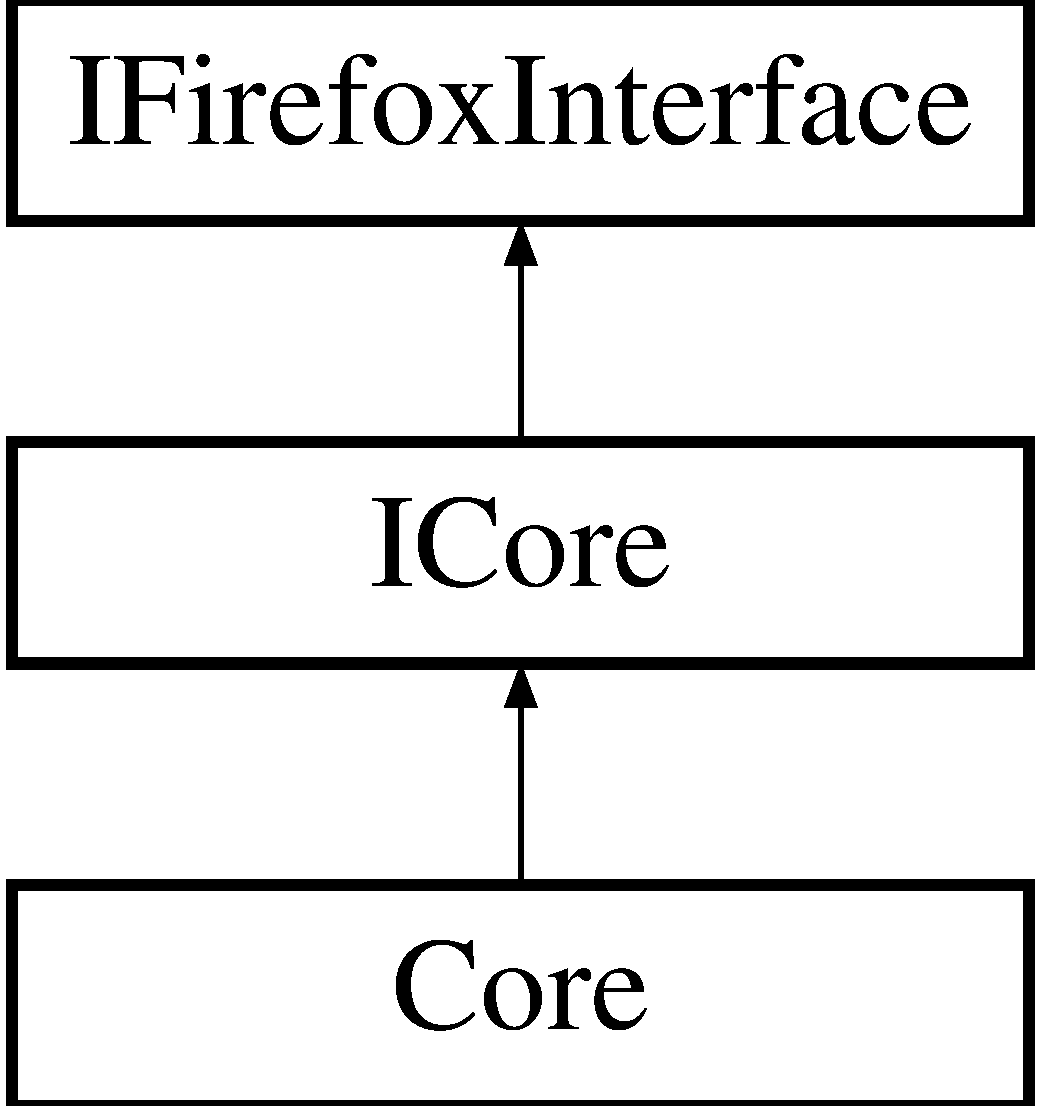
\includegraphics[height=3.000000cm]{classefb_1_1IFirefoxInterface}
\end{center}
\end{figure}
\subsection*{Public Member Functions}
\begin{DoxyCompactItemize}
\item 
virtual unsigned int \hyperlink{classefb_1_1IFirefoxInterface_acd3325eac068a6e4a32dbd8bdf50d54b}{initialise} ()=0
\begin{DoxyCompactList}\small\item\em Initialise library with Facebook ID and extension directory. \item\end{DoxyCompactList}\item 
virtual void \hyperlink{classefb_1_1IFirefoxInterface_af6ee7eacbde6b379b68d954e44f6e549}{close} ()=0
\begin{DoxyCompactList}\small\item\em Close the library and wipe any volatile directories. \item\end{DoxyCompactList}\item 
virtual unsigned int \hyperlink{classefb_1_1IFirefoxInterface_ad827d43af3181b0b177817da74e873d8}{encryptFileInImage} (const \hyperlink{structefb_1_1FacebookId}{FacebookId} ids\mbox{[}$\,$\mbox{]}, const unsigned int len, const char $\ast$src\_\-filename, const char $\ast$img\_\-out\_\-filename) const =0
\begin{DoxyCompactList}\small\item\em Encrypt a file into an image for the supplied array of recipients. \item\end{DoxyCompactList}\item 
virtual unsigned int \hyperlink{classefb_1_1IFirefoxInterface_aaa517bbc318bd8032e01bea927032349}{decryptFileFromImage} (const char $\ast$img\_\-in\_\-filename, const char $\ast$dst\_\-filename) const =0
\begin{DoxyCompactList}\small\item\em Attempt to extract and decrypt a file from an image. \item\end{DoxyCompactList}\item 
virtual unsigned int \hyperlink{classefb_1_1IFirefoxInterface_aea1ea8467fe1857814a0842180b2379d}{encryptString} (const char $\ast$input, char $\ast$output) const =0
\begin{DoxyCompactList}\small\item\em Take a message string and encrypt into a Facebook-\/ready string. Both will be null terminated. \item\end{DoxyCompactList}\item 
virtual unsigned int \hyperlink{classefb_1_1IFirefoxInterface_afcfa5352da3bbca19d3ebde053db9faa}{decryptString} (const char $\ast$input, char $\ast$output) const =0
\begin{DoxyCompactList}\small\item\em Take string from Facebook and decrypt to a message string. Both will be null terminated. \item\end{DoxyCompactList}\item 
virtual unsigned int \hyperlink{classefb_1_1IFirefoxInterface_ab6ba711ad3ecdedf7e968abcdd1ebc58}{calculateBitErrorRate} (const char $\ast$file1, const char $\ast$file2) const =0
\begin{DoxyCompactList}\small\item\em Debug function for calculating BER. \item\end{DoxyCompactList}\end{DoxyCompactItemize}


\subsection{Detailed Description}
Firefox interface definition. 

\subsection{Member Function Documentation}
\hypertarget{classefb_1_1IFirefoxInterface_acd3325eac068a6e4a32dbd8bdf50d54b}{
\index{efb::IFirefoxInterface@{efb::IFirefoxInterface}!initialise@{initialise}}
\index{initialise@{initialise}!efb::IFirefoxInterface@{efb::IFirefoxInterface}}
\subsubsection[{initialise}]{\setlength{\rightskip}{0pt plus 5cm}virtual unsigned int initialise (
\begin{DoxyParamCaption}
{}
\end{DoxyParamCaption}
)\hspace{0.3cm}{\ttfamily  \mbox{[}pure virtual\mbox{]}}}}
\label{classefb_1_1IFirefoxInterface_acd3325eac068a6e4a32dbd8bdf50d54b}


Initialise library with Facebook ID and extension directory. 

\hypertarget{classefb_1_1IFirefoxInterface_af6ee7eacbde6b379b68d954e44f6e549}{
\index{efb::IFirefoxInterface@{efb::IFirefoxInterface}!close@{close}}
\index{close@{close}!efb::IFirefoxInterface@{efb::IFirefoxInterface}}
\subsubsection[{close}]{\setlength{\rightskip}{0pt plus 5cm}virtual void close (
\begin{DoxyParamCaption}
{}
\end{DoxyParamCaption}
)\hspace{0.3cm}{\ttfamily  \mbox{[}pure virtual\mbox{]}}}}
\label{classefb_1_1IFirefoxInterface_af6ee7eacbde6b379b68d954e44f6e549}


Close the library and wipe any volatile directories. 

\hypertarget{classefb_1_1IFirefoxInterface_ad827d43af3181b0b177817da74e873d8}{
\index{efb::IFirefoxInterface@{efb::IFirefoxInterface}!encryptFileInImage@{encryptFileInImage}}
\index{encryptFileInImage@{encryptFileInImage}!efb::IFirefoxInterface@{efb::IFirefoxInterface}}
\subsubsection[{encryptFileInImage}]{\setlength{\rightskip}{0pt plus 5cm}virtual unsigned int encryptFileInImage (
\begin{DoxyParamCaption}
\item[{const {\bf FacebookId}}]{ ids\mbox{[}$\,$\mbox{]}, }
\item[{const unsigned int}]{ len, }
\item[{const char $\ast$}]{ src\_\-filename, }
\item[{const char $\ast$}]{ img\_\-out\_\-filename}
\end{DoxyParamCaption}
) const\hspace{0.3cm}{\ttfamily  \mbox{[}pure virtual\mbox{]}}}}
\label{classefb_1_1IFirefoxInterface_ad827d43af3181b0b177817da74e873d8}


Encrypt a file into an image for the supplied array of recipients. 

\hypertarget{classefb_1_1IFirefoxInterface_aaa517bbc318bd8032e01bea927032349}{
\index{efb::IFirefoxInterface@{efb::IFirefoxInterface}!decryptFileFromImage@{decryptFileFromImage}}
\index{decryptFileFromImage@{decryptFileFromImage}!efb::IFirefoxInterface@{efb::IFirefoxInterface}}
\subsubsection[{decryptFileFromImage}]{\setlength{\rightskip}{0pt plus 5cm}virtual unsigned int decryptFileFromImage (
\begin{DoxyParamCaption}
\item[{const char $\ast$}]{ img\_\-in\_\-filename, }
\item[{const char $\ast$}]{ dst\_\-filename}
\end{DoxyParamCaption}
) const\hspace{0.3cm}{\ttfamily  \mbox{[}pure virtual\mbox{]}}}}
\label{classefb_1_1IFirefoxInterface_aaa517bbc318bd8032e01bea927032349}


Attempt to extract and decrypt a file from an image. 

\hypertarget{classefb_1_1IFirefoxInterface_aea1ea8467fe1857814a0842180b2379d}{
\index{efb::IFirefoxInterface@{efb::IFirefoxInterface}!encryptString@{encryptString}}
\index{encryptString@{encryptString}!efb::IFirefoxInterface@{efb::IFirefoxInterface}}
\subsubsection[{encryptString}]{\setlength{\rightskip}{0pt plus 5cm}virtual unsigned int encryptString (
\begin{DoxyParamCaption}
\item[{const char $\ast$}]{ input, }
\item[{char $\ast$}]{ output}
\end{DoxyParamCaption}
) const\hspace{0.3cm}{\ttfamily  \mbox{[}pure virtual\mbox{]}}}}
\label{classefb_1_1IFirefoxInterface_aea1ea8467fe1857814a0842180b2379d}


Take a message string and encrypt into a Facebook-\/ready string. Both will be null terminated. 

\hypertarget{classefb_1_1IFirefoxInterface_afcfa5352da3bbca19d3ebde053db9faa}{
\index{efb::IFirefoxInterface@{efb::IFirefoxInterface}!decryptString@{decryptString}}
\index{decryptString@{decryptString}!efb::IFirefoxInterface@{efb::IFirefoxInterface}}
\subsubsection[{decryptString}]{\setlength{\rightskip}{0pt plus 5cm}virtual unsigned int decryptString (
\begin{DoxyParamCaption}
\item[{const char $\ast$}]{ input, }
\item[{char $\ast$}]{ output}
\end{DoxyParamCaption}
) const\hspace{0.3cm}{\ttfamily  \mbox{[}pure virtual\mbox{]}}}}
\label{classefb_1_1IFirefoxInterface_afcfa5352da3bbca19d3ebde053db9faa}


Take string from Facebook and decrypt to a message string. Both will be null terminated. 

\hypertarget{classefb_1_1IFirefoxInterface_ab6ba711ad3ecdedf7e968abcdd1ebc58}{
\index{efb::IFirefoxInterface@{efb::IFirefoxInterface}!calculateBitErrorRate@{calculateBitErrorRate}}
\index{calculateBitErrorRate@{calculateBitErrorRate}!efb::IFirefoxInterface@{efb::IFirefoxInterface}}
\subsubsection[{calculateBitErrorRate}]{\setlength{\rightskip}{0pt plus 5cm}virtual unsigned int calculateBitErrorRate (
\begin{DoxyParamCaption}
\item[{const char $\ast$}]{ file1, }
\item[{const char $\ast$}]{ file2}
\end{DoxyParamCaption}
) const\hspace{0.3cm}{\ttfamily  \mbox{[}pure virtual\mbox{]}}}}
\label{classefb_1_1IFirefoxInterface_ab6ba711ad3ecdedf7e968abcdd1ebc58}


Debug function for calculating BER. 


\hypertarget{classefb_1_1ReedSolomon255Fec}{
\section{ReedSolomon255Fec Class Reference}
\label{classefb_1_1ReedSolomon255Fec}\index{efb::ReedSolomon255Fec@{efb::ReedSolomon255Fec}}
}


Reed Solomon error correction using the Schifra library with 255-\/byte block size providing a (255,223) code rate.  


Inheritance diagram for ReedSolomon255Fec:\begin{figure}[H]
\begin{center}
\leavevmode
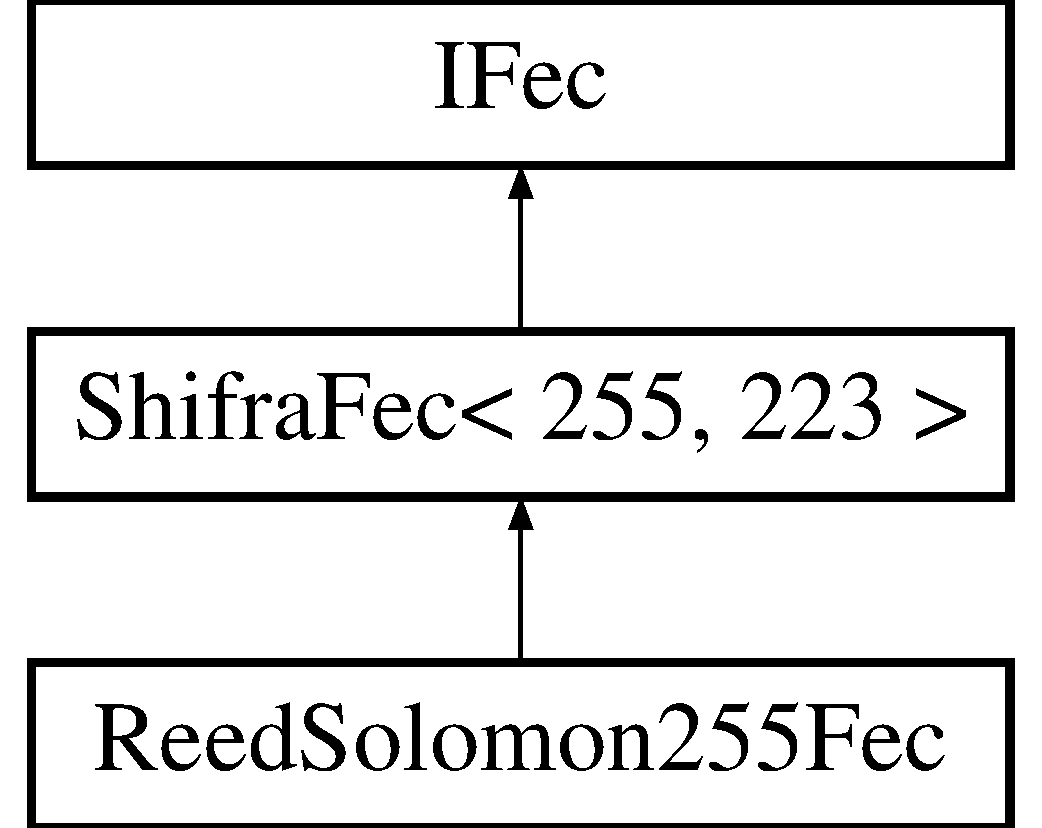
\includegraphics[height=3.000000cm]{classefb_1_1ReedSolomon255Fec}
\end{center}
\end{figure}
\subsection*{Public Member Functions}
\begin{DoxyCompactItemize}
\item 
\hyperlink{classefb_1_1ReedSolomon255Fec_acce4b1484bf84deb14ee0292706764fa}{ReedSolomon255Fec} ()
\begin{DoxyCompactList}\small\item\em Default constructor. \item\end{DoxyCompactList}\end{DoxyCompactItemize}


\subsection{Detailed Description}
Reed Solomon error correction using the Schifra library with 255-\/byte block size providing a (255,223) code rate. 

\subsection{Constructor \& Destructor Documentation}
\hypertarget{classefb_1_1ReedSolomon255Fec_acce4b1484bf84deb14ee0292706764fa}{
\index{efb::ReedSolomon255Fec@{efb::ReedSolomon255Fec}!ReedSolomon255Fec@{ReedSolomon255Fec}}
\index{ReedSolomon255Fec@{ReedSolomon255Fec}!efb::ReedSolomon255Fec@{efb::ReedSolomon255Fec}}
\subsubsection[{ReedSolomon255Fec}]{\setlength{\rightskip}{0pt plus 5cm}{\bf ReedSolomon255Fec} (
\begin{DoxyParamCaption}
{}
\end{DoxyParamCaption}
)}}
\label{classefb_1_1ReedSolomon255Fec_acce4b1484bf84deb14ee0292706764fa}


Default constructor. 


\hypertarget{classefb_1_1ShifraFec}{
\section{ShifraFec$<$ N, M $>$ Class Template Reference}
\label{classefb_1_1ShifraFec}\index{efb::ShifraFec@{efb::ShifraFec}}
}


Shifra Reed Solomon error correction library where code rate is (N,M).  


Inheritance diagram for ShifraFec$<$ N, M $>$:\begin{figure}[H]
\begin{center}
\leavevmode
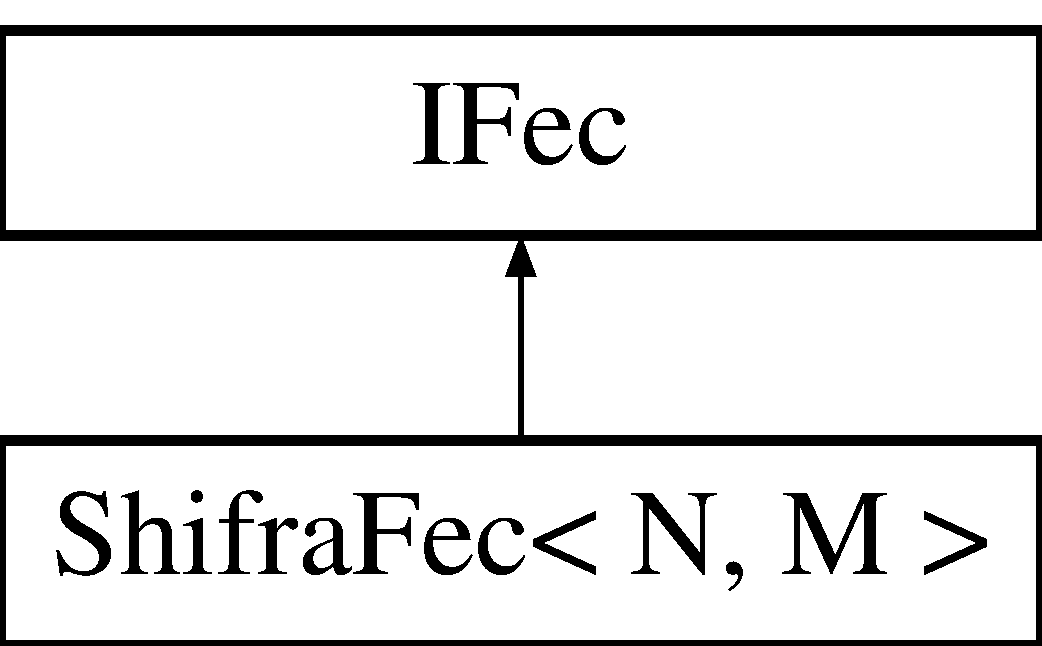
\includegraphics[height=2.000000cm]{classefb_1_1ShifraFec}
\end{center}
\end{figure}
\subsection*{Public Member Functions}
\begin{DoxyCompactItemize}
\item 
\hyperlink{classefb_1_1ShifraFec_a5423cbbbac1657aaa4869a56f57c7812}{ShifraFec} (std::size\_\-t field\_\-descriptor, std::size\_\-t generator\_\-polynommial\_\-index, std::size\_\-t generator\_\-polynommial\_\-root\_\-count)
\begin{DoxyCompactList}\small\item\em Default constructor. \item\end{DoxyCompactList}\end{DoxyCompactItemize}
\subsection*{Private Member Functions}
\begin{DoxyCompactItemize}
\item 
void \hyperlink{classefb_1_1ShifraFec_abfa614d594bf4d7c86b6a8817f35dec5}{encodeBlock} (std::string \&message, std::string \&fec) const 
\begin{DoxyCompactList}\small\item\em Generate FEC code from a message. \item\end{DoxyCompactList}\item 
void \hyperlink{classefb_1_1ShifraFec_a00958e2a880e71ba6a8b6a0e8f560c45}{decodeBlock} (std::string \&message\_\-plus\_\-errors, std::string \&fec, std::string \&message) const 
\begin{DoxyCompactList}\small\item\em Try and fix any errors in a block-\/size message using FEC code. \item\end{DoxyCompactList}\end{DoxyCompactItemize}
\subsection*{Private Attributes}
\begin{DoxyCompactItemize}
\item 
const std::size\_\-t \hyperlink{classefb_1_1ShifraFec_aab1a6051362d9a8b9dc1bf66162743ba}{field\_\-descriptor\_\-}
\item 
const std::size\_\-t \hyperlink{classefb_1_1ShifraFec_a0151caad93dcee8fd76042845c7761d1}{generator\_\-polynommial\_\-index\_\-}
\item 
const std::size\_\-t \hyperlink{classefb_1_1ShifraFec_a187b4bde8c8d1626ee351ad9d8a10efb}{generator\_\-polynommial\_\-root\_\-count\_\-}
\item 
const std::size\_\-t \hyperlink{classefb_1_1ShifraFec_aec880d94a65f32e64736d21ecc62caee}{code\_\-length\_\-}
\item 
const std::size\_\-t \hyperlink{classefb_1_1ShifraFec_a560cb28c8a918c24356967a3c35604ad}{fec\_\-length\_\-}
\item 
const std::size\_\-t \hyperlink{classefb_1_1ShifraFec_a780eb0b73c725bab3470002b4746d07e}{data\_\-length\_\-}
\item 
schifra::galois::field \hyperlink{classefb_1_1ShifraFec_a770e111002e7a8b19041c4f3a972b2c1}{field\_\-}
\item 
schifra::galois::field\_\-polynomial \hyperlink{classefb_1_1ShifraFec_a80fe940d7742c12811d27cbb50d605dc}{generator\_\-polynomial\_\-}
\item 
schifra::sequential\_\-root\_\-generator\_\-polynomial\_\-creator \hyperlink{classefb_1_1ShifraFec_a6dd291fa5e301f1d88eba72e486c22d3}{polynomial\_\-creator\_\-}
\item 
schifra::reed\_\-solomon::encoder$<$ N, M-\/N $>$ \hyperlink{classefb_1_1ShifraFec_a48add19c7145ddef42b214f772508c0f}{encoder\_\-}
\item 
schifra::reed\_\-solomon::decoder$<$ N, M-\/N $>$ \hyperlink{classefb_1_1ShifraFec_acddab8a0f72a511d8b03ffecfe77735a}{decoder\_\-}
\end{DoxyCompactItemize}


\subsection{Detailed Description}
\subsubsection*{template$<$int N, int M$>$ class efb::ShifraFec$<$ N, M $>$}

Shifra Reed Solomon error correction library where code rate is (N,M). 

\subsection{Constructor \& Destructor Documentation}
\hypertarget{classefb_1_1ShifraFec_a5423cbbbac1657aaa4869a56f57c7812}{
\index{efb::ShifraFec@{efb::ShifraFec}!ShifraFec@{ShifraFec}}
\index{ShifraFec@{ShifraFec}!efb::ShifraFec@{efb::ShifraFec}}
\subsubsection[{ShifraFec}]{\setlength{\rightskip}{0pt plus 5cm}{\bf ShifraFec} (
\begin{DoxyParamCaption}
\item[{std::size\_\-t}]{ field\_\-descriptor, }
\item[{std::size\_\-t}]{ generator\_\-polynommial\_\-index, }
\item[{std::size\_\-t}]{ generator\_\-polynommial\_\-root\_\-count}
\end{DoxyParamCaption}
)}}
\label{classefb_1_1ShifraFec_a5423cbbbac1657aaa4869a56f57c7812}


Default constructor. 



\subsection{Member Function Documentation}
\hypertarget{classefb_1_1ShifraFec_abfa614d594bf4d7c86b6a8817f35dec5}{
\index{efb::ShifraFec@{efb::ShifraFec}!encodeBlock@{encodeBlock}}
\index{encodeBlock@{encodeBlock}!efb::ShifraFec@{efb::ShifraFec}}
\subsubsection[{encodeBlock}]{\setlength{\rightskip}{0pt plus 5cm}void encodeBlock (
\begin{DoxyParamCaption}
\item[{std::string \&}]{ message, }
\item[{std::string \&}]{ fec}
\end{DoxyParamCaption}
) const\hspace{0.3cm}{\ttfamily  \mbox{[}private\mbox{]}}}}
\label{classefb_1_1ShifraFec_abfa614d594bf4d7c86b6a8817f35dec5}


Generate FEC code from a message. 

\hypertarget{classefb_1_1ShifraFec_a00958e2a880e71ba6a8b6a0e8f560c45}{
\index{efb::ShifraFec@{efb::ShifraFec}!decodeBlock@{decodeBlock}}
\index{decodeBlock@{decodeBlock}!efb::ShifraFec@{efb::ShifraFec}}
\subsubsection[{decodeBlock}]{\setlength{\rightskip}{0pt plus 5cm}void decodeBlock (
\begin{DoxyParamCaption}
\item[{std::string \&}]{ message\_\-plus\_\-errors, }
\item[{std::string \&}]{ fec, }
\item[{std::string \&}]{ message}
\end{DoxyParamCaption}
) const\hspace{0.3cm}{\ttfamily  \mbox{[}private\mbox{]}}}}
\label{classefb_1_1ShifraFec_a00958e2a880e71ba6a8b6a0e8f560c45}


Try and fix any errors in a block-\/size message using FEC code. 



\subsection{Member Data Documentation}
\hypertarget{classefb_1_1ShifraFec_aab1a6051362d9a8b9dc1bf66162743ba}{
\index{efb::ShifraFec@{efb::ShifraFec}!field\_\-descriptor\_\-@{field\_\-descriptor\_\-}}
\index{field\_\-descriptor\_\-@{field\_\-descriptor\_\-}!efb::ShifraFec@{efb::ShifraFec}}
\subsubsection[{field\_\-descriptor\_\-}]{\setlength{\rightskip}{0pt plus 5cm}const std::size\_\-t {\bf field\_\-descriptor\_\-}\hspace{0.3cm}{\ttfamily  \mbox{[}private\mbox{]}}}}
\label{classefb_1_1ShifraFec_aab1a6051362d9a8b9dc1bf66162743ba}
\hypertarget{classefb_1_1ShifraFec_a0151caad93dcee8fd76042845c7761d1}{
\index{efb::ShifraFec@{efb::ShifraFec}!generator\_\-polynommial\_\-index\_\-@{generator\_\-polynommial\_\-index\_\-}}
\index{generator\_\-polynommial\_\-index\_\-@{generator\_\-polynommial\_\-index\_\-}!efb::ShifraFec@{efb::ShifraFec}}
\subsubsection[{generator\_\-polynommial\_\-index\_\-}]{\setlength{\rightskip}{0pt plus 5cm}const std::size\_\-t {\bf generator\_\-polynommial\_\-index\_\-}\hspace{0.3cm}{\ttfamily  \mbox{[}private\mbox{]}}}}
\label{classefb_1_1ShifraFec_a0151caad93dcee8fd76042845c7761d1}
\hypertarget{classefb_1_1ShifraFec_a187b4bde8c8d1626ee351ad9d8a10efb}{
\index{efb::ShifraFec@{efb::ShifraFec}!generator\_\-polynommial\_\-root\_\-count\_\-@{generator\_\-polynommial\_\-root\_\-count\_\-}}
\index{generator\_\-polynommial\_\-root\_\-count\_\-@{generator\_\-polynommial\_\-root\_\-count\_\-}!efb::ShifraFec@{efb::ShifraFec}}
\subsubsection[{generator\_\-polynommial\_\-root\_\-count\_\-}]{\setlength{\rightskip}{0pt plus 5cm}const std::size\_\-t {\bf generator\_\-polynommial\_\-root\_\-count\_\-}\hspace{0.3cm}{\ttfamily  \mbox{[}private\mbox{]}}}}
\label{classefb_1_1ShifraFec_a187b4bde8c8d1626ee351ad9d8a10efb}
\hypertarget{classefb_1_1ShifraFec_aec880d94a65f32e64736d21ecc62caee}{
\index{efb::ShifraFec@{efb::ShifraFec}!code\_\-length\_\-@{code\_\-length\_\-}}
\index{code\_\-length\_\-@{code\_\-length\_\-}!efb::ShifraFec@{efb::ShifraFec}}
\subsubsection[{code\_\-length\_\-}]{\setlength{\rightskip}{0pt plus 5cm}const std::size\_\-t {\bf code\_\-length\_\-}\hspace{0.3cm}{\ttfamily  \mbox{[}private\mbox{]}}}}
\label{classefb_1_1ShifraFec_aec880d94a65f32e64736d21ecc62caee}
\hypertarget{classefb_1_1ShifraFec_a560cb28c8a918c24356967a3c35604ad}{
\index{efb::ShifraFec@{efb::ShifraFec}!fec\_\-length\_\-@{fec\_\-length\_\-}}
\index{fec\_\-length\_\-@{fec\_\-length\_\-}!efb::ShifraFec@{efb::ShifraFec}}
\subsubsection[{fec\_\-length\_\-}]{\setlength{\rightskip}{0pt plus 5cm}const std::size\_\-t {\bf fec\_\-length\_\-}\hspace{0.3cm}{\ttfamily  \mbox{[}private\mbox{]}}}}
\label{classefb_1_1ShifraFec_a560cb28c8a918c24356967a3c35604ad}
\hypertarget{classefb_1_1ShifraFec_a780eb0b73c725bab3470002b4746d07e}{
\index{efb::ShifraFec@{efb::ShifraFec}!data\_\-length\_\-@{data\_\-length\_\-}}
\index{data\_\-length\_\-@{data\_\-length\_\-}!efb::ShifraFec@{efb::ShifraFec}}
\subsubsection[{data\_\-length\_\-}]{\setlength{\rightskip}{0pt plus 5cm}const std::size\_\-t {\bf data\_\-length\_\-}\hspace{0.3cm}{\ttfamily  \mbox{[}private\mbox{]}}}}
\label{classefb_1_1ShifraFec_a780eb0b73c725bab3470002b4746d07e}
\hypertarget{classefb_1_1ShifraFec_a770e111002e7a8b19041c4f3a972b2c1}{
\index{efb::ShifraFec@{efb::ShifraFec}!field\_\-@{field\_\-}}
\index{field\_\-@{field\_\-}!efb::ShifraFec@{efb::ShifraFec}}
\subsubsection[{field\_\-}]{\setlength{\rightskip}{0pt plus 5cm}schifra::galois::field {\bf field\_\-}\hspace{0.3cm}{\ttfamily  \mbox{[}private\mbox{]}}}}
\label{classefb_1_1ShifraFec_a770e111002e7a8b19041c4f3a972b2c1}
\hypertarget{classefb_1_1ShifraFec_a80fe940d7742c12811d27cbb50d605dc}{
\index{efb::ShifraFec@{efb::ShifraFec}!generator\_\-polynomial\_\-@{generator\_\-polynomial\_\-}}
\index{generator\_\-polynomial\_\-@{generator\_\-polynomial\_\-}!efb::ShifraFec@{efb::ShifraFec}}
\subsubsection[{generator\_\-polynomial\_\-}]{\setlength{\rightskip}{0pt plus 5cm}schifra::galois::field\_\-polynomial {\bf generator\_\-polynomial\_\-}\hspace{0.3cm}{\ttfamily  \mbox{[}private\mbox{]}}}}
\label{classefb_1_1ShifraFec_a80fe940d7742c12811d27cbb50d605dc}
\hypertarget{classefb_1_1ShifraFec_a6dd291fa5e301f1d88eba72e486c22d3}{
\index{efb::ShifraFec@{efb::ShifraFec}!polynomial\_\-creator\_\-@{polynomial\_\-creator\_\-}}
\index{polynomial\_\-creator\_\-@{polynomial\_\-creator\_\-}!efb::ShifraFec@{efb::ShifraFec}}
\subsubsection[{polynomial\_\-creator\_\-}]{\setlength{\rightskip}{0pt plus 5cm}schifra::sequential\_\-root\_\-generator\_\-polynomial\_\-creator {\bf polynomial\_\-creator\_\-}\hspace{0.3cm}{\ttfamily  \mbox{[}private\mbox{]}}}}
\label{classefb_1_1ShifraFec_a6dd291fa5e301f1d88eba72e486c22d3}
\hypertarget{classefb_1_1ShifraFec_a48add19c7145ddef42b214f772508c0f}{
\index{efb::ShifraFec@{efb::ShifraFec}!encoder\_\-@{encoder\_\-}}
\index{encoder\_\-@{encoder\_\-}!efb::ShifraFec@{efb::ShifraFec}}
\subsubsection[{encoder\_\-}]{\setlength{\rightskip}{0pt plus 5cm}schifra::reed\_\-solomon::encoder$<$N,M-\/N$>$ {\bf encoder\_\-}\hspace{0.3cm}{\ttfamily  \mbox{[}private\mbox{]}}}}
\label{classefb_1_1ShifraFec_a48add19c7145ddef42b214f772508c0f}
\hypertarget{classefb_1_1ShifraFec_acddab8a0f72a511d8b03ffecfe77735a}{
\index{efb::ShifraFec@{efb::ShifraFec}!decoder\_\-@{decoder\_\-}}
\index{decoder\_\-@{decoder\_\-}!efb::ShifraFec@{efb::ShifraFec}}
\subsubsection[{decoder\_\-}]{\setlength{\rightskip}{0pt plus 5cm}schifra::reed\_\-solomon::decoder$<$N,M-\/N$>$ {\bf decoder\_\-}\hspace{0.3cm}{\ttfamily  \mbox{[}private\mbox{]}}}}
\label{classefb_1_1ShifraFec_acddab8a0f72a511d8b03ffecfe77735a}

\printindex
\end{document}
